\documentclass{article}

%Um mit Latex zu arbeiten braucht man zwei Dinge:
% https://miktex.org/download
% https://www.xm1math.net/texmaker/download.html

%Hilfreiche Links:
%Sonderzeichen in Latex einfügen: https://de.wikibooks.org/wiki/LaTeX-Kompendium:_Sonderzeichen

\usepackage{xcolor}
\usepackage{graphicx}
\usepackage{listings}
\usepackage{float}
\usepackage{url}
\usepackage{verbatim}
\usepackage{multirow}
\usepackage{comment}
\usepackage{mathtools}
\usepackage[section]{placeins}
\usepackage{amsmath}
\usepackage{ulem}
\usepackage{cancel}
\newcommand{\mbeq}{\overset{!}{=}}
\DeclarePairedDelimiter\abs{\lvert}{\rvert}%

%% Better Listings
%\usepackage{xcolor}
%\definecolor{LightGray}{gray}{.9}
%\usepackage{minted}

\begin{document} 

\begin{titlepage}
\title{Gaussian beam optics}
%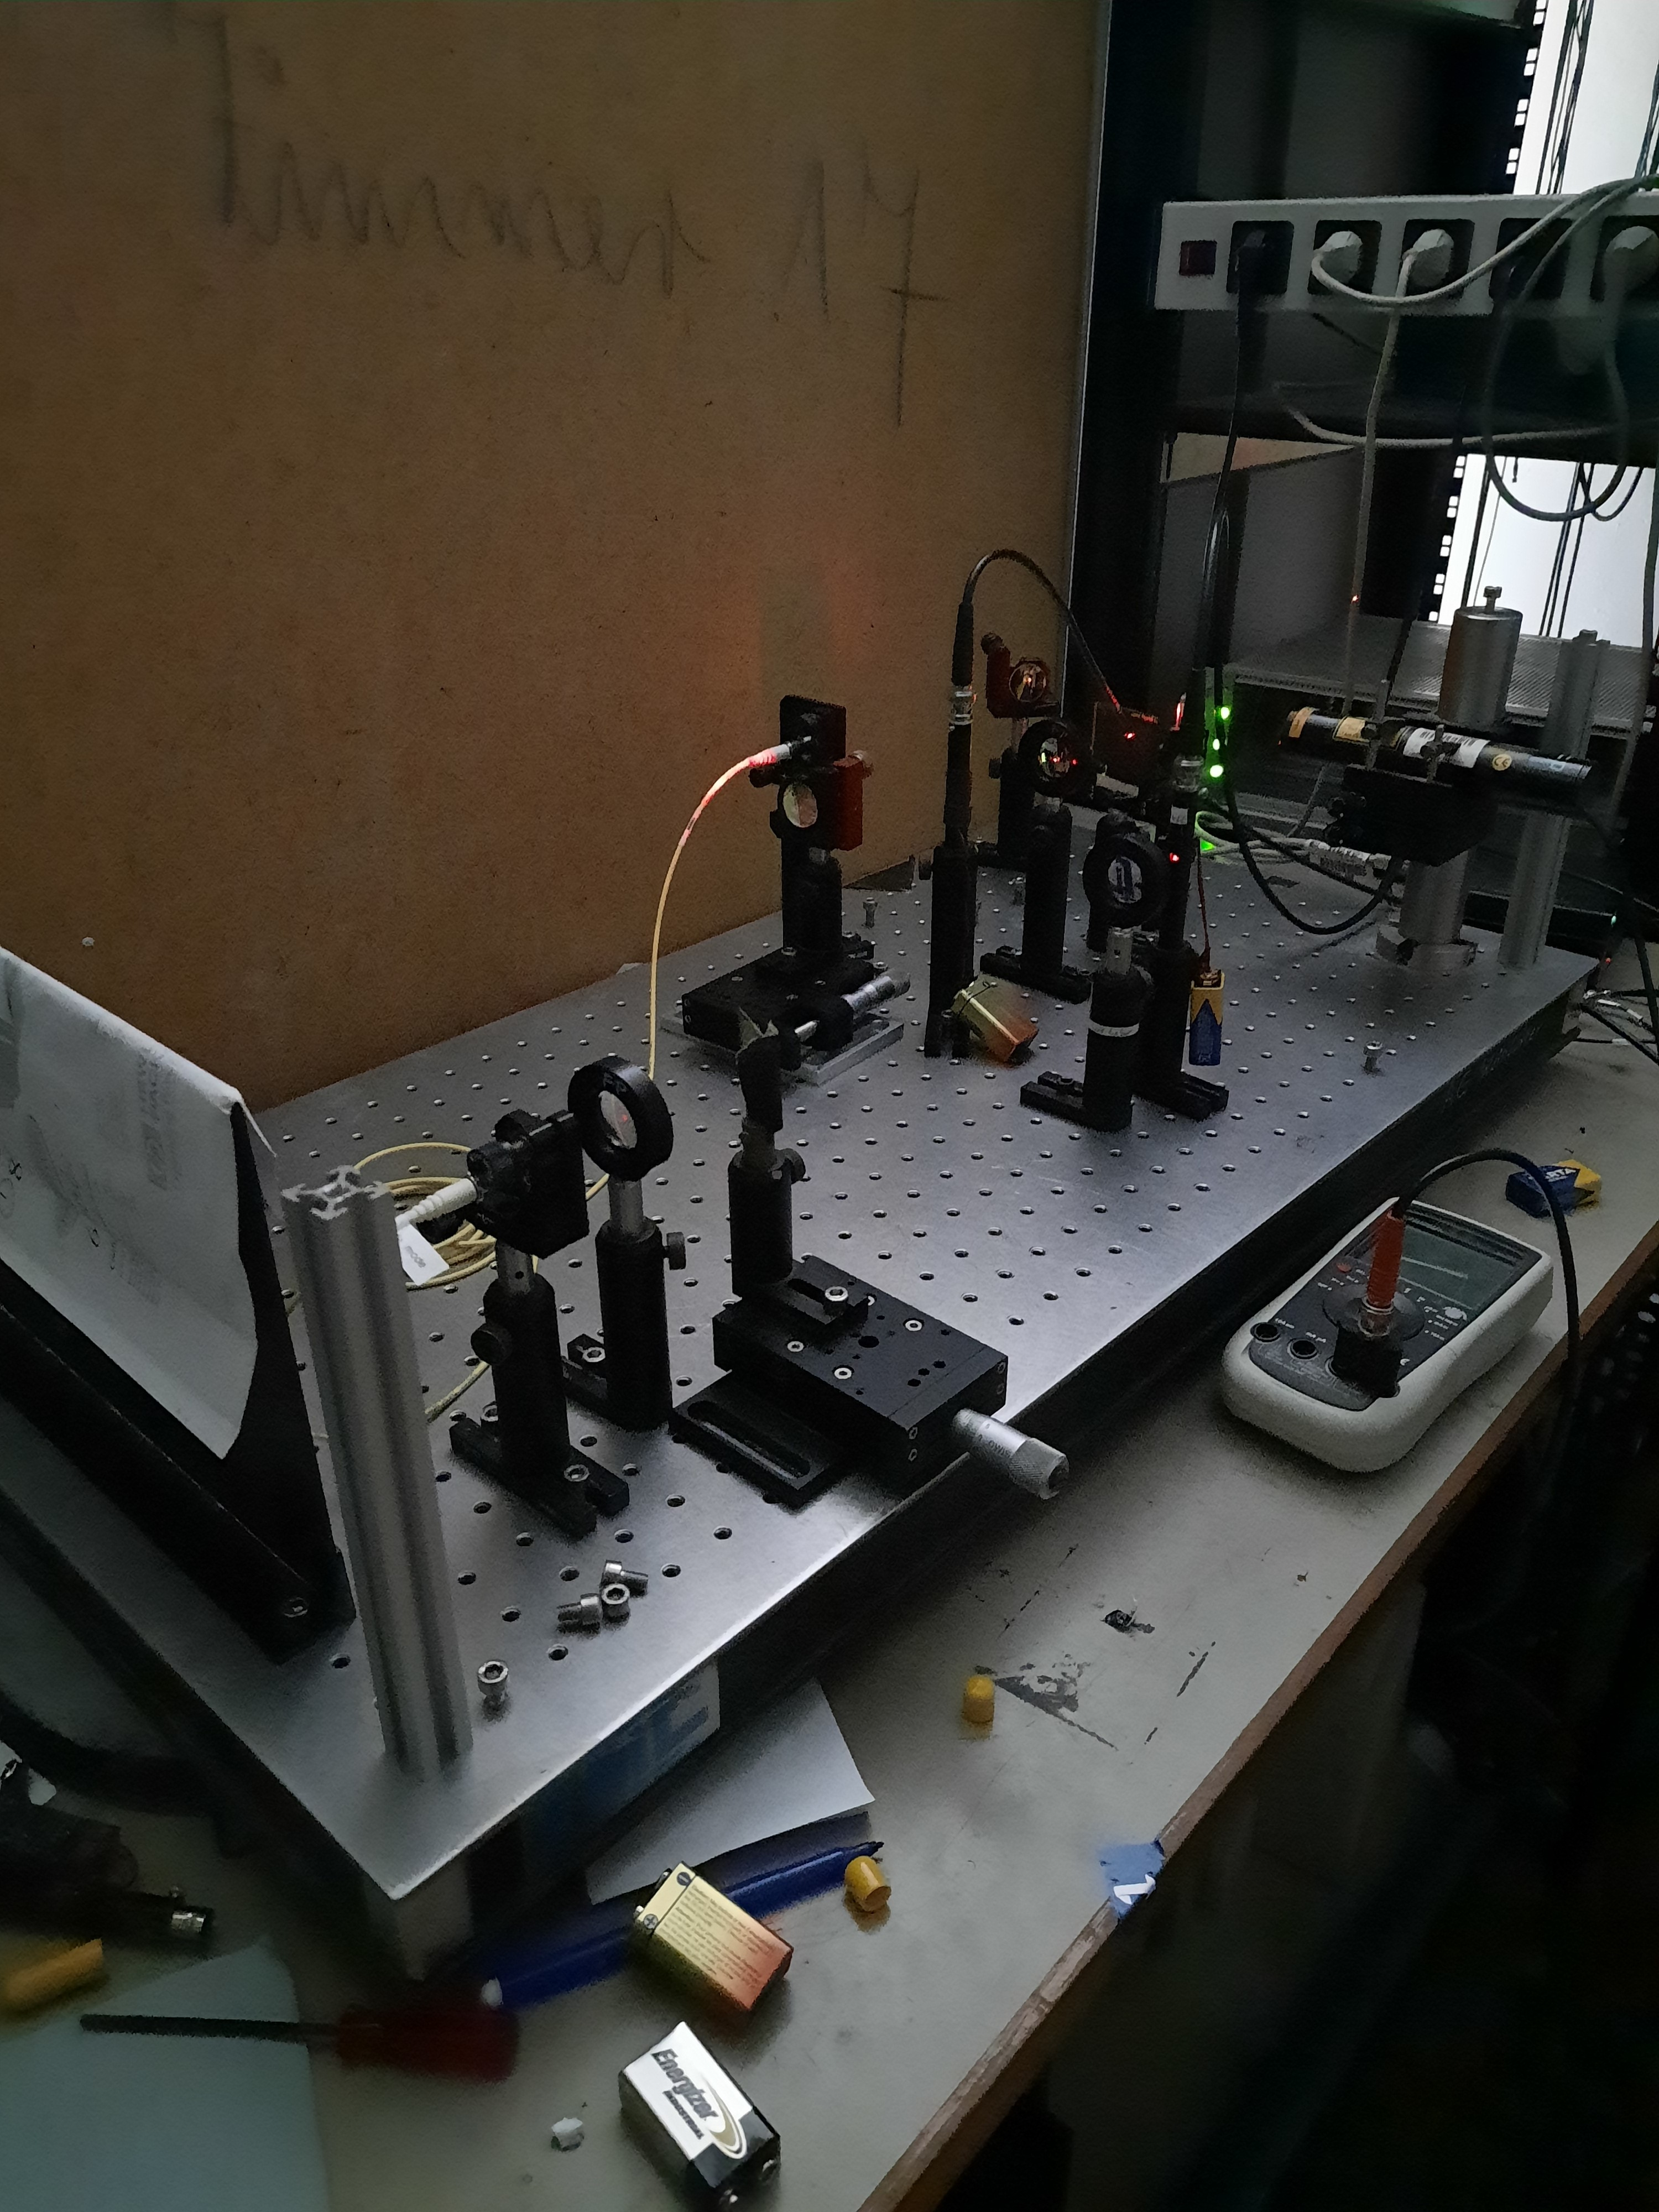
\includegraphics[\textwidth]{TV3-aufbau.jpg}
\author{Corinna Elena Wegner, Garen Gregorian}
\date{June 8, 2022}
\maketitle %hiermit wird das Deckblatt erst erstellt
\end{titlepage}

\newpage
\tableofcontents
\newpage

\section{Introduction} 
%Wenn ich \subsection* schreibe (mit *), kommt diese Überschrift nicht in die Gliederung

In this experiment, the properties of a gaussian beam were investigated using photodiodes and a Fabry-Perot interferometer.
\\
\textcolor{red}{übersetzen und noch mehr schreiben??}
\textcolor{red}{Genereller Versuchsaufbau mit Skizze}

\subsection{Problems from the experimental instructions}

We are asked to calculate the necessary distance between two lenses in order to change the waist of a given gaussian beam to a given value.

Representing the propagation of the beam through our optical system using transfermatrices:

 $M = M_{f_2}M_{Prop}M_{f_1}=\begin{pmatrix}1 & 0\\ \frac{-1}{f_2} & 1
\end{pmatrix}\begin{pmatrix}1 & L\\ 0 & 1
\end{pmatrix}\begin{pmatrix}1 & 0\\ \frac{-1}{f_1} & 1
\end{pmatrix} =\begin{pmatrix}1 & 0\\ \frac{-1}{f_2} & 1
\end{pmatrix}\begin{pmatrix} 1-\frac{L}{f_2} & L\\ \frac{-1}{f_2} & 1
\end{pmatrix} = \begin{pmatrix} 1-\frac{L}{f_2} & L\\ \frac{-1}{f_2}+\frac{L}{f_2 f_2}-\frac{1}{f_2} & 1-\frac{L}{f_2}
\end{pmatrix}
 = \begin{pmatrix} A&B\\C&D\end{pmatrix}$

\setlength{\parskip}{2em}

q' and q are defined as:
$
q=0+iz_r$\par$
{q}'={z}'+i{z_r}'
$

And using the ABCD rule for gaussian beams on q' we get: 
${q}'=\frac{Aq+B}{Cq+D}=\frac{iz_r(1-\frac{L}{f_1})+L}{iz_r(\frac{L}{f_1 f_2}-\frac{1}{f_1}-\frac{1}{f_2})+1-\frac{L}{f_2}}=\frac{i\frac{\pi\omega_0^2}{\lambda}(1-\frac{L}{f_1})+L}{i\frac{\pi\omega_0^2}{\lambda}(\frac{L}{f_1 f_2}-\frac{1}{f_1}-\frac{1}{f_2})+1-\frac{L}{f_2}}\mbeq i\frac{\pi\omega_0^2}{\lambda}+{z}'$ 


For a general quotient of complex numbers:

$\frac{ai+b}{{a}'i+{b}'}=\frac{(ai+b)(-{a}'i+b)}{({a}'i+{b}')(-{a}'i+{b}')}=\frac{a{a}'+b{b}'+i(a{b}'-{a}'b)}{{a}'^2+{b}'^2}
$

$\Rightarrow{} {q}' = \frac{b{b}'+z_r^2(1-\frac{L}{f_1})(\frac{L}{f_1 f_2}-\frac{1}{f_2}-\frac{1}{f_1})}{z_r^2(\frac{L}{f_1 f_2})-\frac{1}{f_2})^2+(1-\frac{L}{f_2})^2}+i\frac{z_r(1-\frac{L}{f_1})(1-\frac{L}{f_2})-z_r(\frac{L}{f_1 f_2}-\frac{1}{f_2}-\frac{1}{f_1})L}{z_r^2(\frac{L}{f_1 f_2}-\frac{1}{f_2}-\frac{1}{f_1})^2+(1-\frac{L}{f_2})^2}
$

$\Rightarrow{} {z}'\mbeq \frac{b{b}'+z_r^2(1-\frac{L}{f_1})(\frac{L}{f_1 f_2}-\frac{1}{f_2}-\frac{1}{f_1})}{z_r^2(\frac{L}{f_1 f_2})-\frac{1}{f_2})^2+(1-\frac{L}{f_2})^2} $
 and
 $\Rightarrow{}{} {z_r}' \frac{z_r(1-\frac{L}{f_1})(1-\frac{L}{f_2})-z_r(\frac{L}{f_1 f_2}-\frac{1}{f_2}-\frac{1}{f_1})L}{z_r^2(\frac{L}{f_1 f_2}-\frac{1}{f_2}-\frac{1}{f_1})^2+(1-\frac{L}{f_2})^2}$
 
 Thus to determine ${z_r}'$
 
 ${z_r}'=z_r\frac{(1-\cancel{\frac{L}{f_2}}-\cancel{\frac{L}{f_1}}+\cancel{\frac{L^2}{f_2 f_1}}-\cancel{\frac{L^2}{f_2 f_1}}+\cancel{\frac{L}{f_2}}+\cancel{\frac{L}{f_1}})}{z_r^2(\frac{L}{f_1 f_2}-\frac{1}{f_1}-\frac{1}{f_2})^2+(1+\frac{1}{f_2})^2}=\frac{z_r}{z_r^2(z_r^2(\frac{L}{f_1 f_2}-\frac{1}{f_1}-\frac{1}{f_2})^2+(1+\frac{1}{f_2})^2)} 
 $
 
 using the attached python code, this yields
 
 $L \approx 0,35 m$


\paragraph{Problem 16}

 In the task on page 16 we were asked to calculate the theoretical values for the experiment on optical resonators. We were given $R=50mm$ for both plano-convex lenses, $L=45mm$ distance between the lenses. The lenses have a width $b=6.35mm$ and a refraction index $n_{L} = 1.515$ The wavelength of the light will be $\lambda = 632nm$ for the following calculations.\\
\\

Upon hitting the first mirror, for the light we have in Matrix representation
\\\\
$M_{boundary 1}= \begin{pmatrix}
1 & 0\\
D_{12}& 1
\end{pmatrix}$ with $D_{12} = -\frac{n_{mirror 1}-n_{air}}{R}$
\\\\
Then for propagation through the first mirror
\\\\
$M_{propagation 1}= \begin{pmatrix}
1 & \frac{b_1}{n_{mirror 1}}\\
0 & 1
\end{pmatrix}$
\\\\
When leaving the mirror
\\\\
$M_{boundary 2}= \begin{pmatrix}
1 & 0\\
D_{23} & 1
\end{pmatrix}$ with $D_{23} = -\frac{n_{air}-n_{mirror 1}}{R'}$
\\\\
Thus in total we have
$M_{mirror 1}= M_{boundary 1} \cdot M_{propagation 1} \cdot M_{boundary 2} 
\\\\
= \begin{pmatrix}
1 & 0\\
D_{12} & 1
\end{pmatrix} \cdot \begin{pmatrix}
1 & \frac{b_1}{n_{mirror 1}}\\
0 & 1
\end{pmatrix} \cdot \begin{pmatrix}
1 & 0\\
D_{23} & 1
\end{pmatrix}= \begin{pmatrix}
\frac{n_2-b \cdot D_{23}}{n_2} & \frac{b}{n_2}\\
-\frac{-D_{12} \cdot n_2 - D_{23}(-D_{12}b+n_2)}{n_2} & \frac{-D_{12}b+n_2}{n_2}
\end{pmatrix}$
\\\\
Since, $n_{mirror1} = n_{mirror 2} \equiv n_2$ and $D_{12} = \frac{n_{mirror 1}-n_{air}}{R}$ and $R \xrightarrow[]{} \infty$ for the first square boundary, $D_{12} \xrightarrow[]{} 0$

$\Rightarrow{} M_{mirror 1}=\begin{pmatrix}
\frac{n_2-b \cdot D_{23}}{n_2} & \frac{b}{n_2}\\
\frac{D_{23}n_2}{n_2} & 1
\end{pmatrix}$
\\
Applying the same method to the second mirror
\\

$M_{mirror 2}= M_{boundary 3} \cdot M_{propagation 2} \cdot M_{boundary 4}$
\\\\
$M_{mirror 2} = \begin{pmatrix}
1 & 0\\
D_{12}' & 1
\end{pmatrix} \cdot \begin{pmatrix}
1 & \frac{b_1}{n_{mirror 1}}\\
0 & 1
\end{pmatrix} \cdot \begin{pmatrix}
1 & 0\\
0 & 1
\end{pmatrix}=\begin{pmatrix}
1 & \frac{b}{n_2}\\
D'_{12} & \frac{D_{23}b+n_2}{n_2}
\end{pmatrix}$
\\
with $ D_{12}' = -\frac{n_{mirror 2}-n_{air}}{R'}$, but this time with a finite $R'$
\\

Therefore, overall
\\\\
$M_{total}= M_{mirror 2} \cdot M'_{prop} \cdot M_{mirror 1}  
\\\\
M_{total}= \begin{pmatrix}
1 & \frac{b}{n_2}\\
D'_{12} & \frac{D_{23}b+n_2}{n_2}
\end{pmatrix}
\cdot
\begin{pmatrix}
1 & 2R'\\
0 & 1
\end{pmatrix} \cdot
\begin{pmatrix}
\frac{n_2-b \cdot D_{23}}{n_2} & \frac{b}{n_2}\\
D_{23} & 1
\end{pmatrix} 
$
\\\\
Now we use $\frac{n-1}{R'} = \frac{1}{f} = 10 m^{-1}, R = 50mm, n=1.515, b=6.35mm $

and calculate
\\\\
$M_{total}= \begin{pmatrix}
2.00 & 0.11\\
30 & 2.08
\end{pmatrix}
$

Using $q = z+iz_R = iz_R$, $z_R = 0.025m$ since $z_R = \frac{\pi \omega^2_0}{\lambda} = \sqrt{\frac{L}{2}(R-\frac{L}{2})}$ since $L=R$ in our confocal arrangement we conclude $z_R=\frac{R}{2}=0.025m$ and thus $q' = \frac{2.00q+0.11}{30q+2.08} = \frac{i2.0(0.025)+0.11}{i30(0.025)+2.08}$
\\\\
Thus:
\\\\
$z'_R = Im(q') = 0.0046692 \approx 4.67\cdot10^{-3}m
\\\\
z' = Re(q') =  0.0536883 \approx 5.37\cdot10^{-2}m
$
\\\\
Hence, we see that the beam has a focus around 5.37 cm after the optical cavity and that the Rayleigh length has decreased considerably, meaning that the beam has further lost collimation.


\section{Measuring the power of the laser}

In the first part we measured the power of the laser itself. First, we put a photodiode with internal resistance 100k$\Omega$
after the first passive reflector and measured the voltage
\ $U=(1.2 \pm 0.1) V$ %So bindet man Formeln in Text ein
. Then we turned the laser off and measured again at the same position to eliminate the background light (the windows were covered by curtains). We measured 
\ $U_b = (1.2 \pm 0.1)mV$ 
using the 
10k$\Omega$
photodiode. 


Though we used a voltmeter, but an Oscilloscope with a known measuring resistance $R_m$ can just as well be used. With the measured voltage $V_m$ one can conclude the photocurrent $I_p = V_m \cdot R_m$. To ensure an accurate measurement, we would want $R_m >>R_i$ since\\

$\frac{1}{R_{total}}= \frac{1}{R_m}+\frac{1}{R_i}$\\

and for sufficiently large $R_i$:\\
$\hspace{3cm}$\\
$\frac{1}{R_{total}} \approx \frac{1}{R_m} \rightarrow R_{total} = R_m$\\


\paragraph{Calculating the power from the voltage}

When the beam hits the diode, the multimeter detects a voltage $U$. For photodiodes, the relation between the power and light current ist given by 
\cite{Quantenausbeute} 
\begin{equation} 
P = \frac{hfI}{e\eta}
\end{equation}
.  
Here, $h = 6.62607015*10^{-34} Js$ is the planck constant, $e = 1.602176634*10^{-19} C$ the charge of an electron, $I$ is the current and $\eta = 0.75$ the quantum efficiency of the photodiode. We can replace the frequency $f$ in the formula by the corresponding wavelength $\lambda = 632.8 nm$ of the laser using $c= \lambda f$, with the vacuum speed of light  $c = 299792458 \frac{m}{s}$. Using ohm's law $ U= R \cdot I$ we eliminate the current $I$ and obtain 
\begin{equation}
P = \frac{hcU}{\lambda Re \eta}
\label{powerfromvoltage}
\end{equation}

The resistance $R$ can be read from the photodiode. In the experiment we used two diodes, mainly diode 1 with $R=10 k\Omega$. Diode 2 has $R= 100 k\Omega$. Thus by plugging the respective values in, we can calculate:
\\

$P_{Laser} =  \frac{6.62607015*10^{-34}\cdot299792458\cdot1.2}{632.8\cdot10^{-9}\cdot1.602176634*10^{-19}\cdot0.75\cdot100000}=3.13*10^{-5} W \vspace{2cm}$


$\Delta P_{Laser}= \pm \frac{6.62607015*10^{-34}\cdot299792458\cdot0.1}{632.8\cdot10^{-9}\cdot1.602176634*10^{-19}\cdot0.75\cdot10^{5}} =\pm 0.27*10^{-5} W\vspace{2cm}$\\

$P_{Background} =  \frac{6.62607015*10^{-34}\cdot299792458\cdot1.2*10^{-3}}{632.8\cdot10^{-9}\cdot1.602176634*10^{-19}\cdot0.75\cdot10^{4}}=0.03*10^{-5}W \vspace{2cm}$\\

$\Delta P_{Background} = \pm \frac{6.62607015*10^{-34}\cdot299792458\cdot0.1}{632.8\cdot10^{-9}\cdot1.602176634*10^{-19}\cdot0.75\cdot10^{5}} =\pm 0.27*10^{-7}W \vspace{2cm}$\\

Thus by subtraction we can determine the power of the laser without any background influence as\\

$P^{'}_{Laser} = 3.13*10^{-5}- 0.03*10^{-5} =3.10*10^{-5} \pm 0.27*10^{-5}W$\\

Since the background power is outside of the measurement error of
the laser power measurement, we cannot ignore the background power, however the difference is so low that one can safely expect results to not change much in a dimmed and normally lit room. A lit room, however, allows for more accurate measurements since observation of scales and thus of measurements becomes easier to the human eye and there are fewer risks of bumping into instruments or the table, thus reducing the chance of misallignments and accidentally influencing measurements.

It is worth noting that imperfections in the fine adjustment of the system or other errors such as dust particles on the diode lenses overall lowered the power output of the laser. Therefore, one can expect the relevance of background power to decrease as the adjustment of the optical system get better.


\section{Coupling the optical fibre cables}

After determining the power of the laser we coupled the fibre optic cables into the coupler in the optical path. First, we coupled the multimode cable and adjusted the optical elements such that the conduction was optimized. By variating the angles a little we tried to see different modes on a piece of paper, put behind the cable. Unlike our expectations we could not identify them, instead the dot on the paper disappeared, because too few light was conducted through the cable. We could however see on the paper a dot with a small dark hole in it's center, just like the shape of a donut mode. It is also possible that the small hole was a dust crumb on the lens whatsoever. Unfortunately it was not possible to take a picture of the dot which shows more than a diffuse point, because the mobile phone cameras could not work with the light conditions.\\

Now we measured the voltage from the photodiode behind the cables. Therefor we focused the beam into the photodiode, using another lens. For the multimode cable we measured a maximum voltage of $U=209mV$, but the value fluctuated a lot (about 20mV just from touching the table). After coupling the single mode cable we measured $U=(106 \pm 5)mV$. This is less than for the multimode cable, which makes sense because there is only one mode lead through the single mode cable. With the resistance of the used photodiode, $R = 10k\Omega$, we can calculate the percentage of the power lead through the cable:\\



The corrected laser power translates to a corrected voltage value for the Laser of \\

$U'_{Laser}= 1.19 \pm 0.11 V$

$\vspace{1cm}$

$U_{single-mode} =(106 \pm 5)mV  \hspace{1cm} U_{multi-mode} = (209\pm 20)mV$

$\vspace{1cm}$

$\eta_{single-mode} = \frac{106}{1.19*10^3} = 8.93\% \hspace{1cm} \eta_{single-mode} = \frac{209}{1.19*10^3} = 17.61\%$

$\vspace{1cm}$

$\Delta\eta_{sinlge-mode} = \pm8.93\%\cdot(\frac{5}{106}+ \frac{0.11}{1.19})= \pm 1.25\%$

$\vspace{1cm}$

$\Delta\eta_{single-mode} =\pm17.61\%\cdot(\frac{20}{209}+\frac{0.11}{1.19})= \pm 3.32\%$

$\vspace{1cm}$

$\xrightarrow[]{} \eta_{single-mode} = 8.93\pm 1.25\%\hspace{1cm}\Delta\eta_{sinlge-mode}=17.61\pm 3.32\%$

$\vspace{1cm}$

As expected, the multi mode cable has a higher efficiency since it allows for more modes to be transmitted. The measured efficiency was highly dependent on the sensitive alignment of the laser. This is especially true for the single mode cable since it has a smaller lens diameter. One can therefore expect misallignment to have lowered the efficiency of the single mode cable more than the multi mode cable. Otherwise, other sources of errors such as imperfect transmission throught the cables or the equipment heating up, which was observed in during the experiments, to have affected both cables equall. The influence of dust particles on the lens of the cables is also noteworthy as a factor that further lowers efficiency.

\section{Measuring the beam profile}

In this experiment we measured the intensity of the laser light that is emitted by the fibre. We cut off some of the beam with a razor blade to see how much voltage is still measured by the photodiode. Thereby we obtained a profile of the beam cross section. After that we put a lens ($f=100mm$) behind the fibre end so that the beam was focused at the focal point. We measured the profile of the beam at different positions between the two lenses (the second lens ($f=50mm$) focuses the beam into the photodiode). Near the focal point of the first lens, where the waist of the gaussian beam lies, we measured three times. To eliminate influences from ambient light, we normalized the voltage signal with the other photodiode.\\

The total power the photodiode is detecting depends on the position of the razor blade $x$ and is given by:
\begin{equation}
P(x) = \int_x^\infty\mathrm{d}x' I_0 \mathrm{e}^{-\frac{2(x'-x_0)^2}{\omega^2}}.
\label{powerintegral}
\end{equation}

\textcolor{red}{Beantworten: Welches Brechungsindexprofil müßte eine Glasfaser aufweisen, damit die Faser eine ideale Gauß-Mode führt?}

\paragraph{Measuring the cross section profile without focusing the beam}

To calculate the beam radius $\omega (z)$ we fitted the data of our measurement a (see appendix) to \ref{powerintegral}. In order to do this we calculated the power from the voltage using \ref{powerfromvoltage}. \\

The output parameters of the fit are:

\begin{tabular}{ccc}
\hline
Label & $I_{0}$ & waist \\ 
\hline
$8.3cm$ & 0.008019362898045088 & 1.829220656900651 \\ 
\hline
$11.0 cm$ & 0.006615023526005974 & -2.7527937817950208 \\ 
\hline
$5.0cm$ & 0.003761871655984494 & 4.766691950975467 \\
\hline
%\label{part_a_results}
\end{tabular}

 For $Distance razor blade - fibre end = 11.0 cm$ the waist is negative, which is impossible and therefore we left this value out in the calculation of the average waist. Since this measurement series was taken at the furthest point from the beam origin, we assume that generally the influence of error sources are much higher than for measurements taken close to the beam origin.\\

The average waist is then $(3.3\pm 1.4) mm$. From that we also calculated the rayleigh length 
\begin{equation}
z_{R} = \frac{\pi\omega_{0}^2 n}{\lambda} 
\label{rayleighlength}
\end{equation}
at which the beam radius is $\sqrt{2}\omega_{0}$. In our case, $n=1$ is the refraction index of the medium (air) and the wavelength of the laser is $\lambda =632.8 nm$. The resulting rayleigh length is:
$65 \pm 48) mm$.\\

\begin{figure}
\includegraphics[width=\textwidth]{part a: cross section profile of collimated beam.png}
\caption{cross section profile of collimated beam}
\label{part_a_fig} %Man kann mit \ref{part_a_fig} auf dieses Bild verweisen
\end{figure}

The first two measurements of the series with $Distance razor blade - fibre end = 8.3 cm$ seemed to fall out of line. When doing the fit, the curve (red dashed) also looked inappropiate. Presumably we measured these points too early, namely not at the point right before the power falls off (i.e. the maximum). Therefore we decided to leave them out of the fitting, which lead to a much better result (see figure \ref{part_a_fig}).

The relatively high errors can be explained by the strong fluctuations of the multimeter display, making it hard to measure the voltage. This can be seen when looking at the following figure, where the measurement points differ quite a lot from the fit curves. However, one can see that the shapes of the fit curves look similar. Another problem of the experiment was that there could be scattering light from the ambient or laser, which influences the photodiode. Furthermore the razor did not really suit the transversal intensity profile of the beam. It only cuts off the beam from one direction, leaving the other direction always open. Therefore there is a systematic error in the experiment. Using an apperture would have been a better way to measure the beam profile. Also, in order to measure at certain distances from the fibre end, we had to put the razor mount into a place between the threads where you can fix the mount on the table. This could lead to a non orthogonal angle between razor and beam, which would mean that you have to turn the micrometer screw more to get the same decrease of intensity. Besides, at the edge of the razor there is diffraction happening, as we have examined in a previous practical. This could also falsify the measurements. At last it was hard to measure the distances in the $z$-direction having only a ruler. The experiment was very barred by the coupler and other optical instruments, so a caliper would have helped to increase the quality of those measurements.

\paragraph{Measuring the cross section profile with lens ($f=100mm$)}

We measured the beam profile using the razor blade technique at seven distances from the lens. Three measurements were taken near the focal point because here we expected the waist $\omega_{0}$, i.e. the minimum of the beam radius $\omega (z)$. They are related by the equation:
\begin{equation}
\omega (z) = \omega_{0}\sqrt{1+\frac{z^2}{z_{R}^2}}
\label{omegaofz}
\end{equation}

The razorblade positions z from which we measured the beam profile are $-(7.0\pm 0.2)cm, -(4.0\pm 0.2)cm, -(1.0\pm 0.2)cm, (0.0\pm 0.2)cm, (1.0\pm 0.2)cm, (4.3\pm 0.2) cm$ and $(7.0\pm 0.2)cm$, where $z=0$ is the focal point. For better clearness we plotted the data near focal point in an extra plot. The plots show the calculated powers (\ref{powerfromvoltage}) from the measuring data along with the corresponding fit to the gaussian integral \ref{powerintegral}. From the fit we obtained $I_{0}$ and $\omega(z)$:

\begin{tabular}{ccc} 
  \hline
  Label & $I_{0}$ & waist \\ 
  \hline
  $-7.0 cm$ &$ 0.006360231677816774$ &$ 1.7189349221192924 $\\ 
  \hline
  $-4.0 cm$ &$ 0.011671364316655813$ &$ 1.1276882272690187 $\\ 
  \hline
  $-1.0cm$ &$ 0.007839724060919795$ &$ 1.440227080283796 $\\
  \hline
  $0.0 cm$ &$ 0.015986220284139128$ &$ 0.9913725114260791 $\\ 
  \hline
  $1.0 cm$ &$ 0.03579668252236531$ &$ 0.252042108041255 $ \\
  \hline
  $4.3 cm$ &$ 0.03333418800700897$ & $ 0.33766227836023854$ \\ 
  \hline
  $7.0 cm$ & $0.0048537944018923511$ & $-2.2479931087206224$\\
  \hline 
%\label{part_b_results}
\end{tabular}

The value $\omega(7cm) = -2.2... $ is negative and therefore illogical. Therefore we left it out from further calculations. Again this measurement series was taken from the furthest point from the fibre end, so we assume generally higher influence from error sources of any kind\\

Again, we fitted the measurement series for each razor-lens-distance $z$ to the \ref{powerintegral} and obtained the local $\omega(z)$. Then we fitted these together with the corresponding $z$ to \ref{omegaofz}.
From that we obtained the waist\\ 
$\omega_{0} = ( 0.8 \pm 0.6 ) mm $\\
The resulting rayleigh length is\\
$z_{R} =  ( 5 \pm 6 ) mm $\\

\begin{figure}[h!]
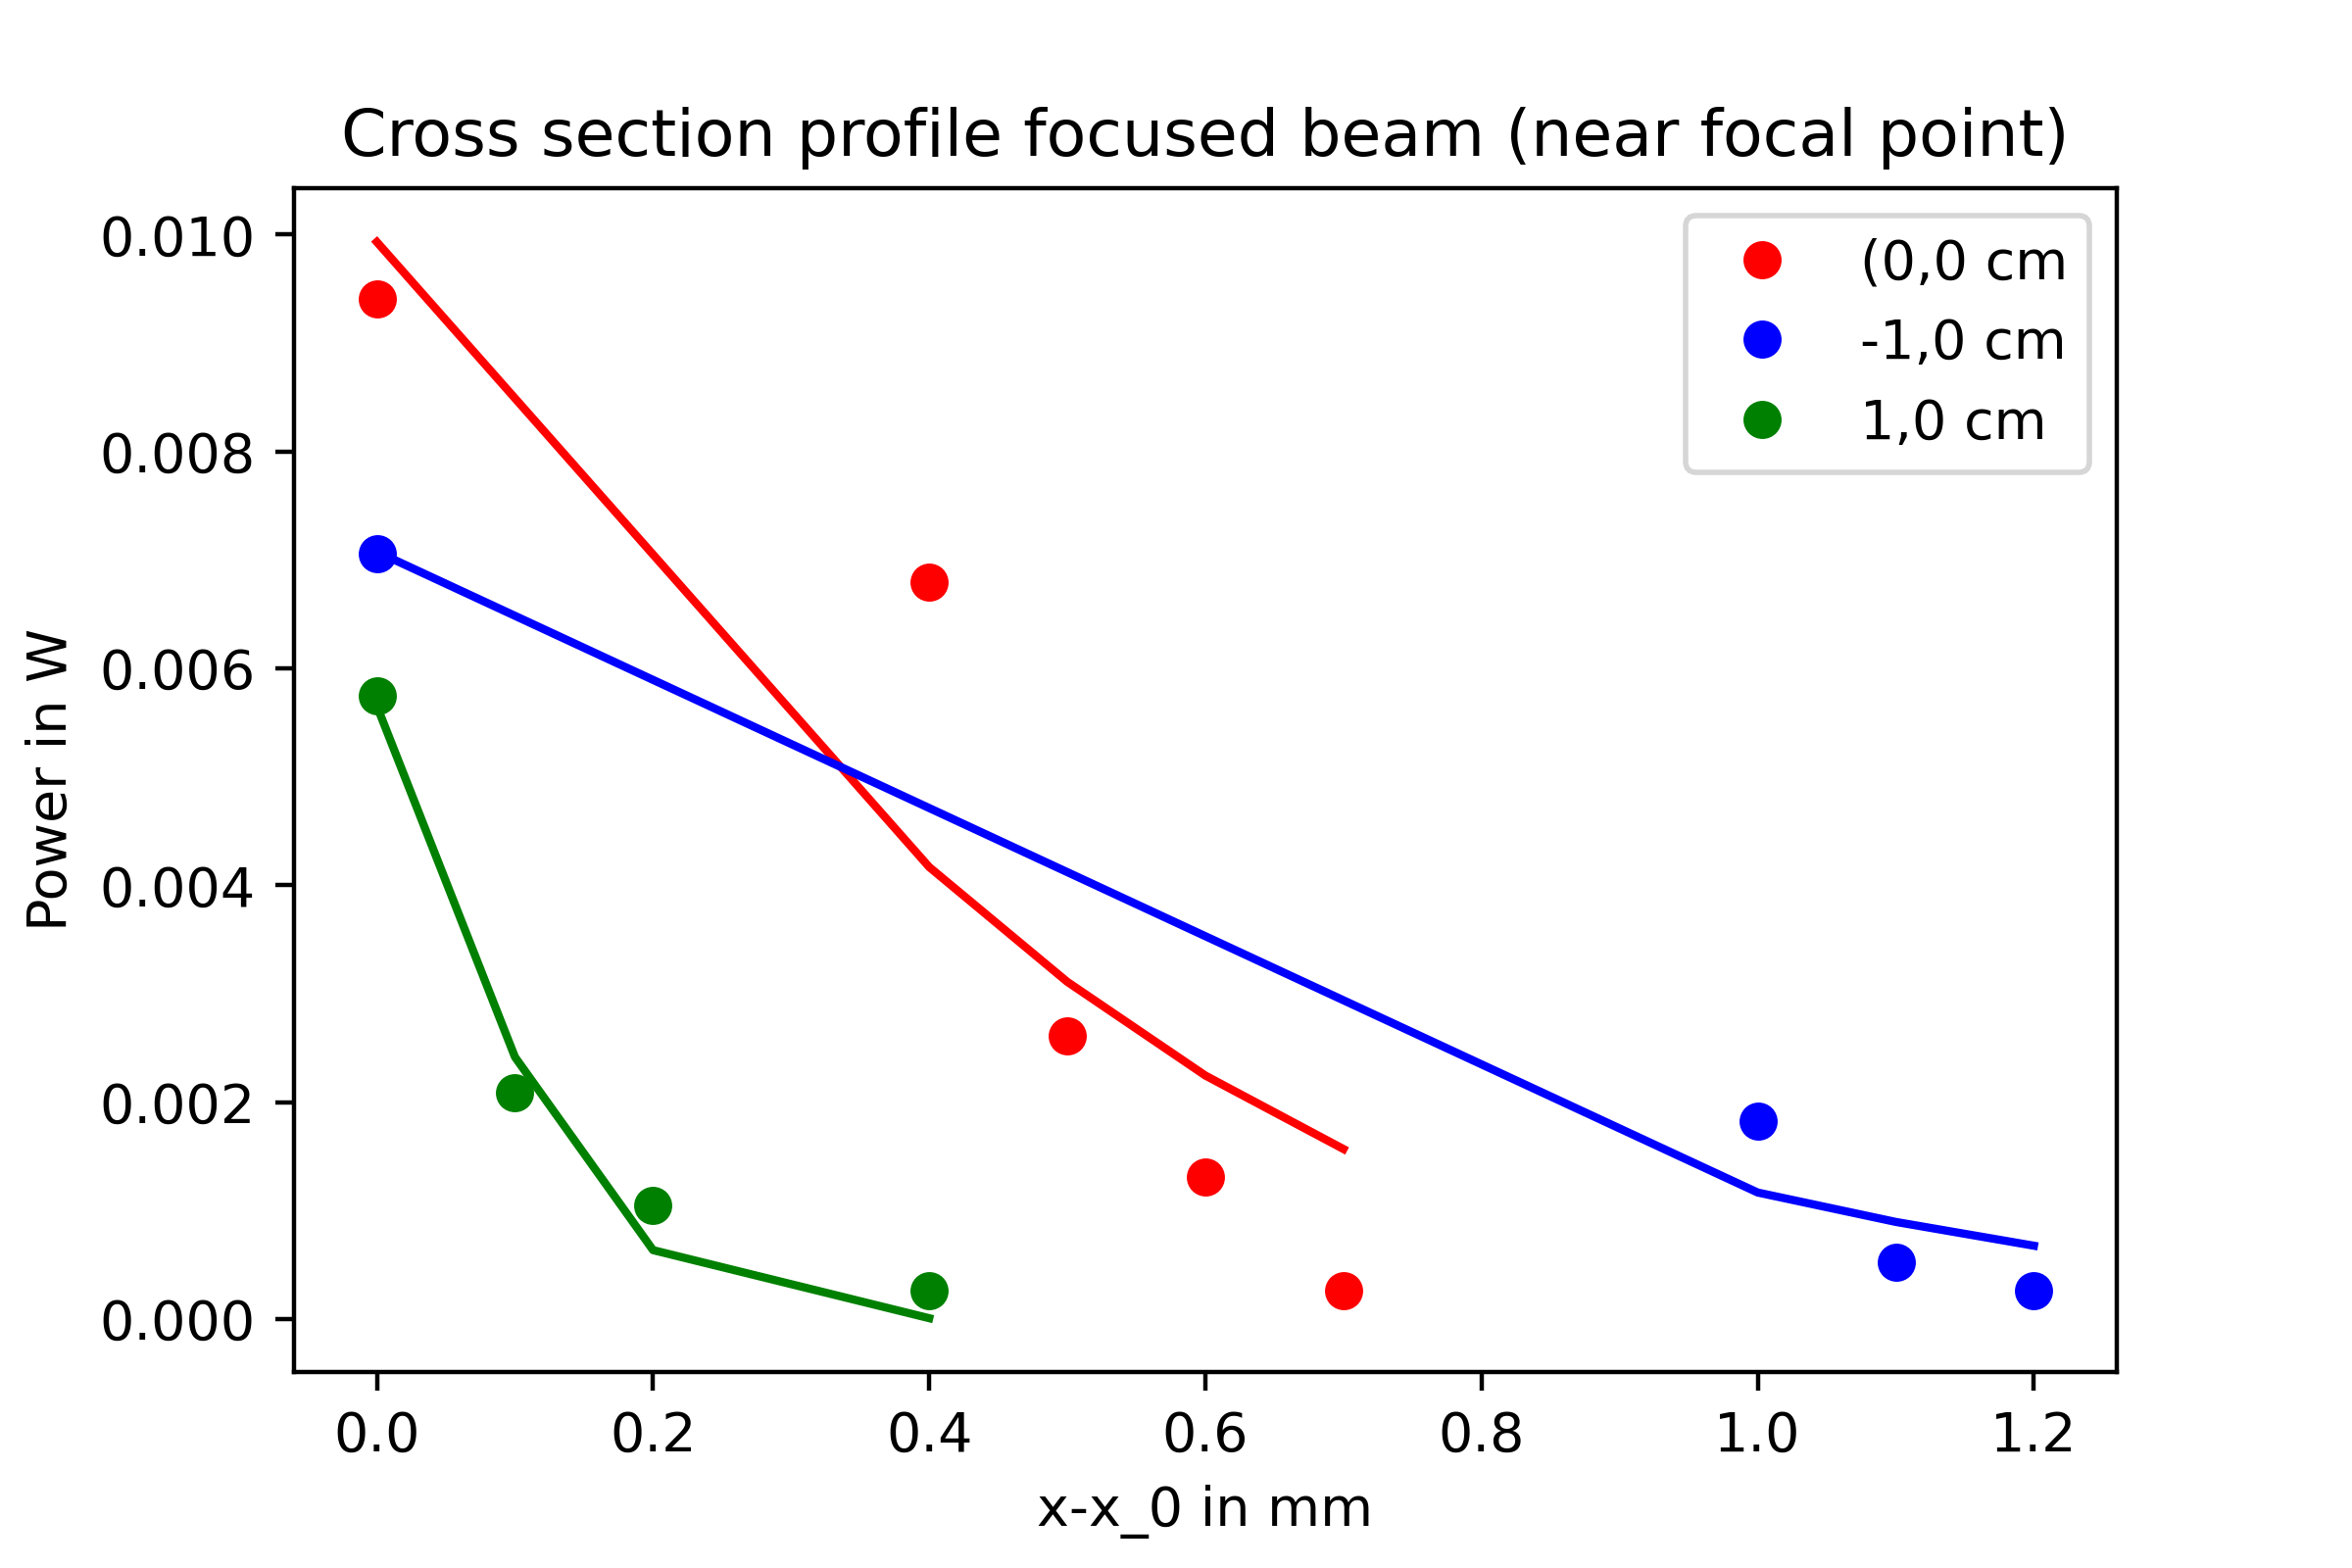
\includegraphics[width=\textwidth]{Cross section profile focused beam (near focal point).png} 
\label{near_focal} 
\end{figure}

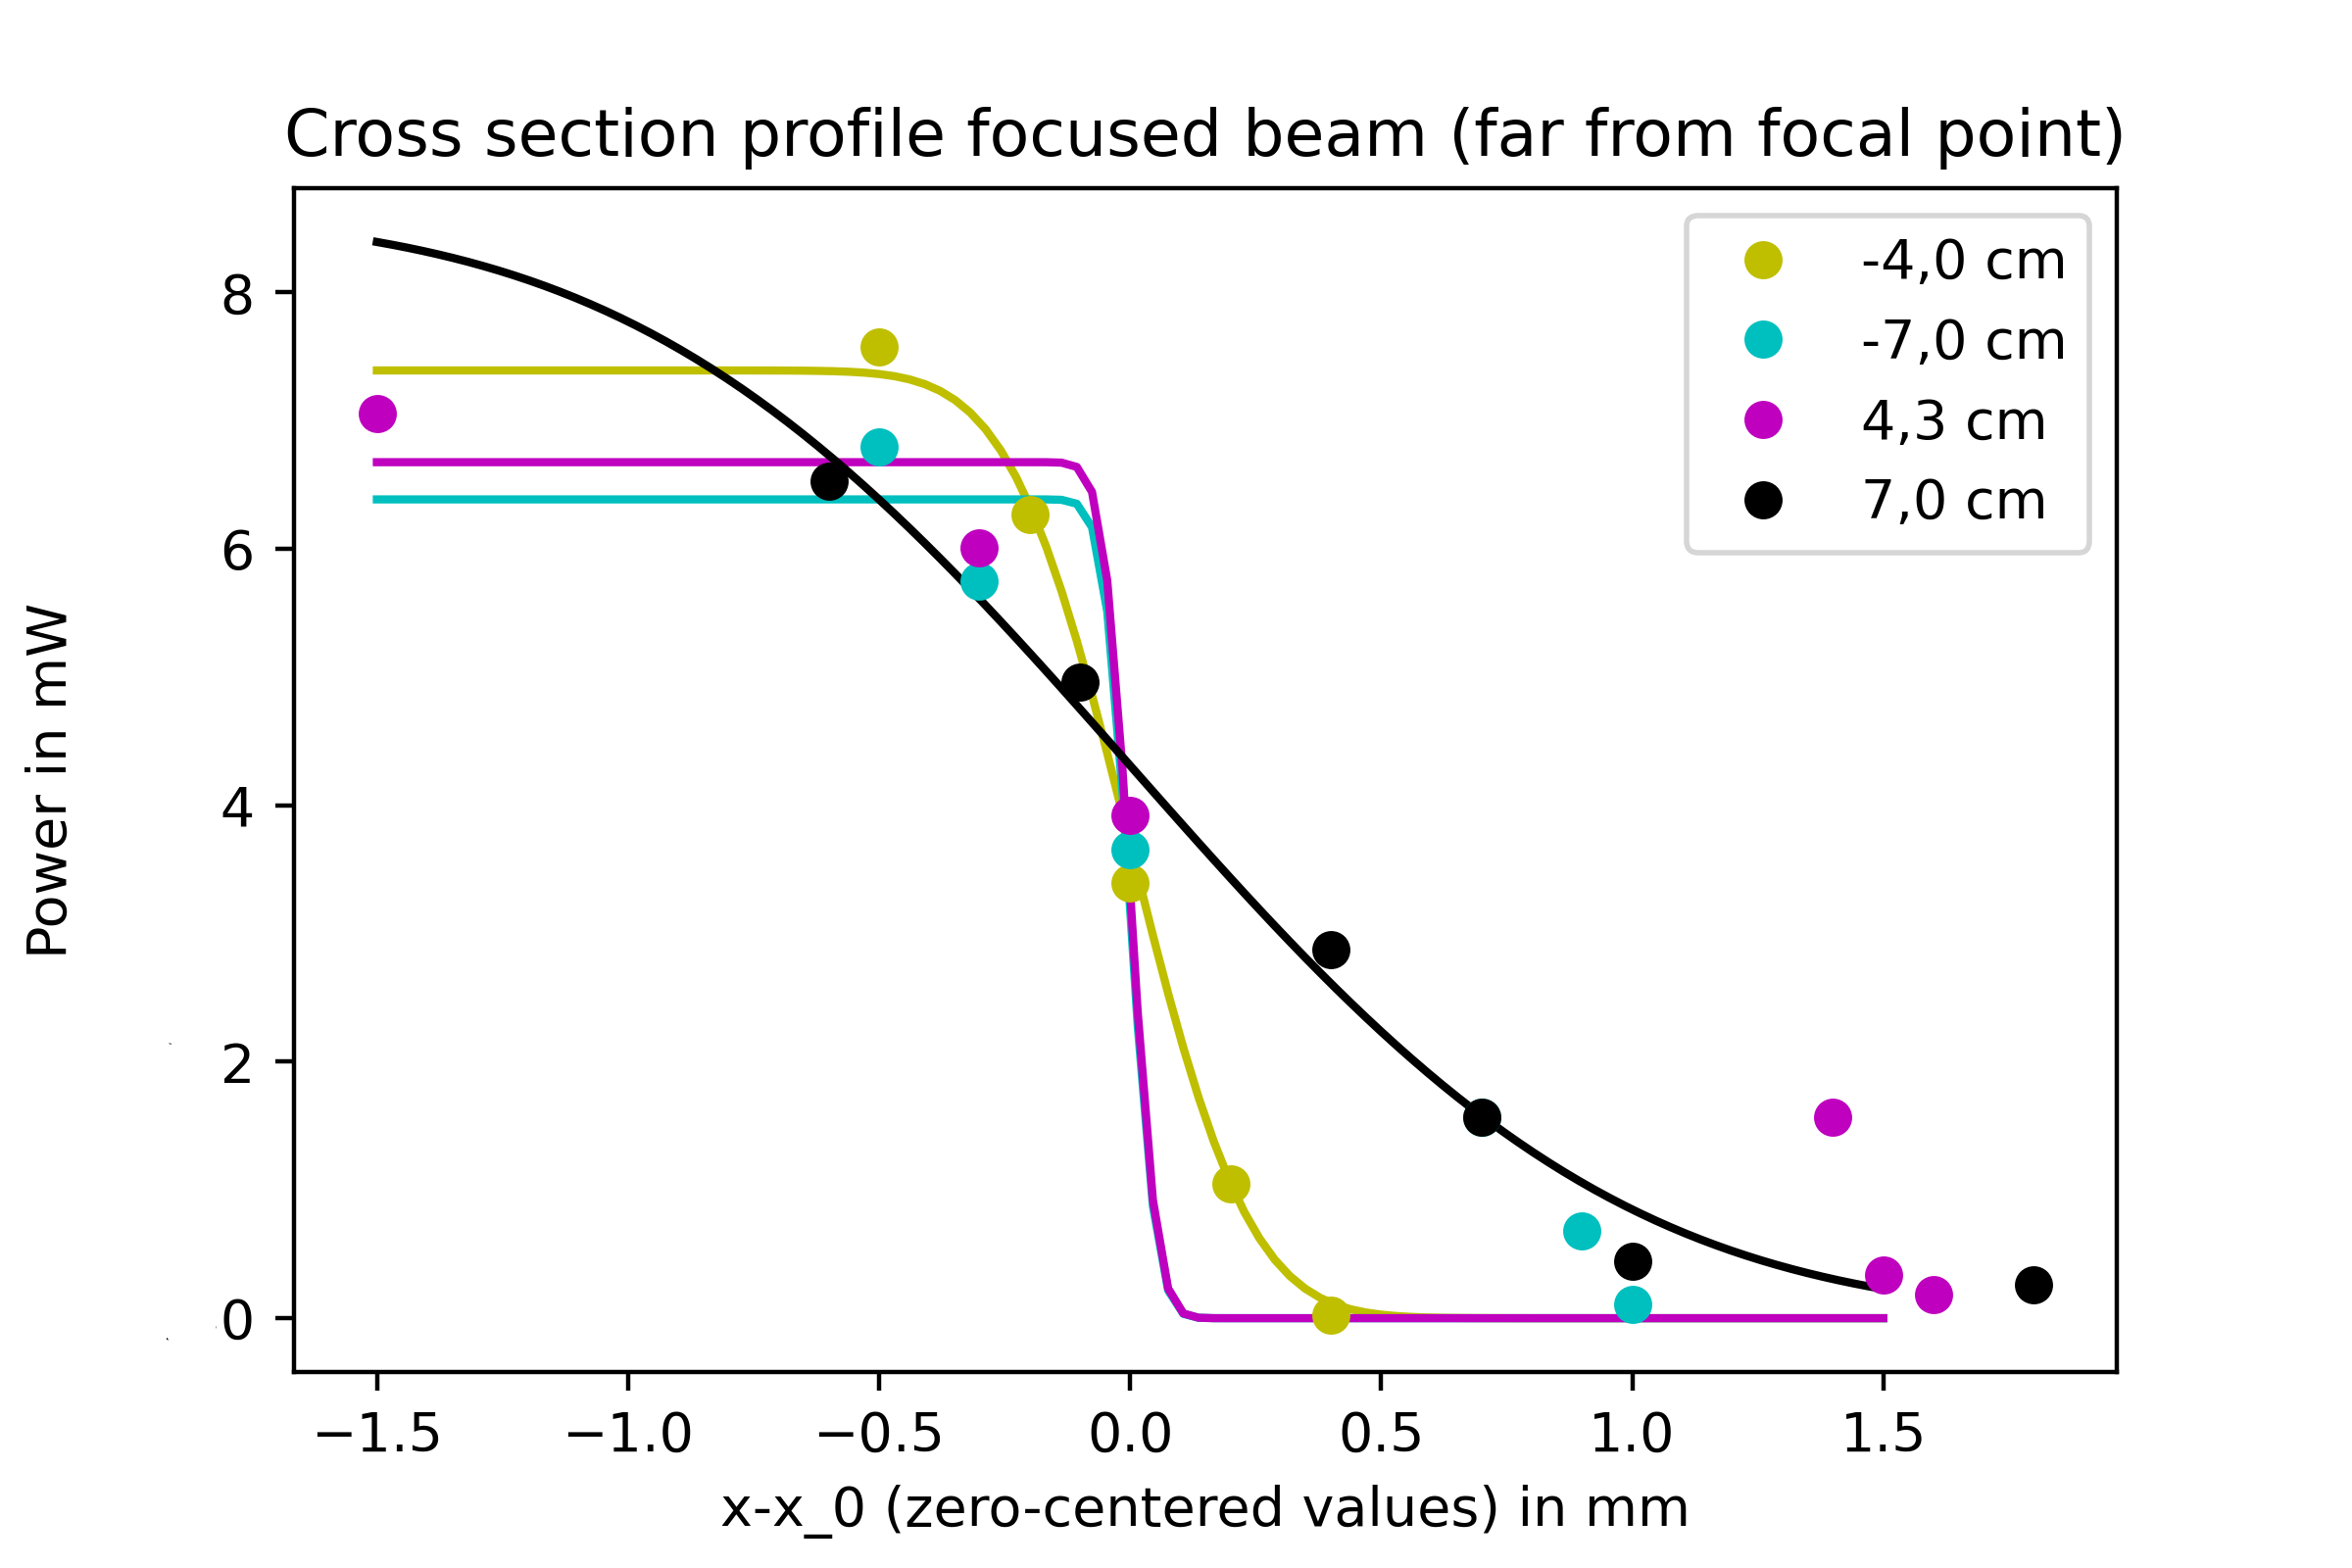
\includegraphics[width=\textwidth]{Cross section profile focused beam (far from focal point).png}[h!]
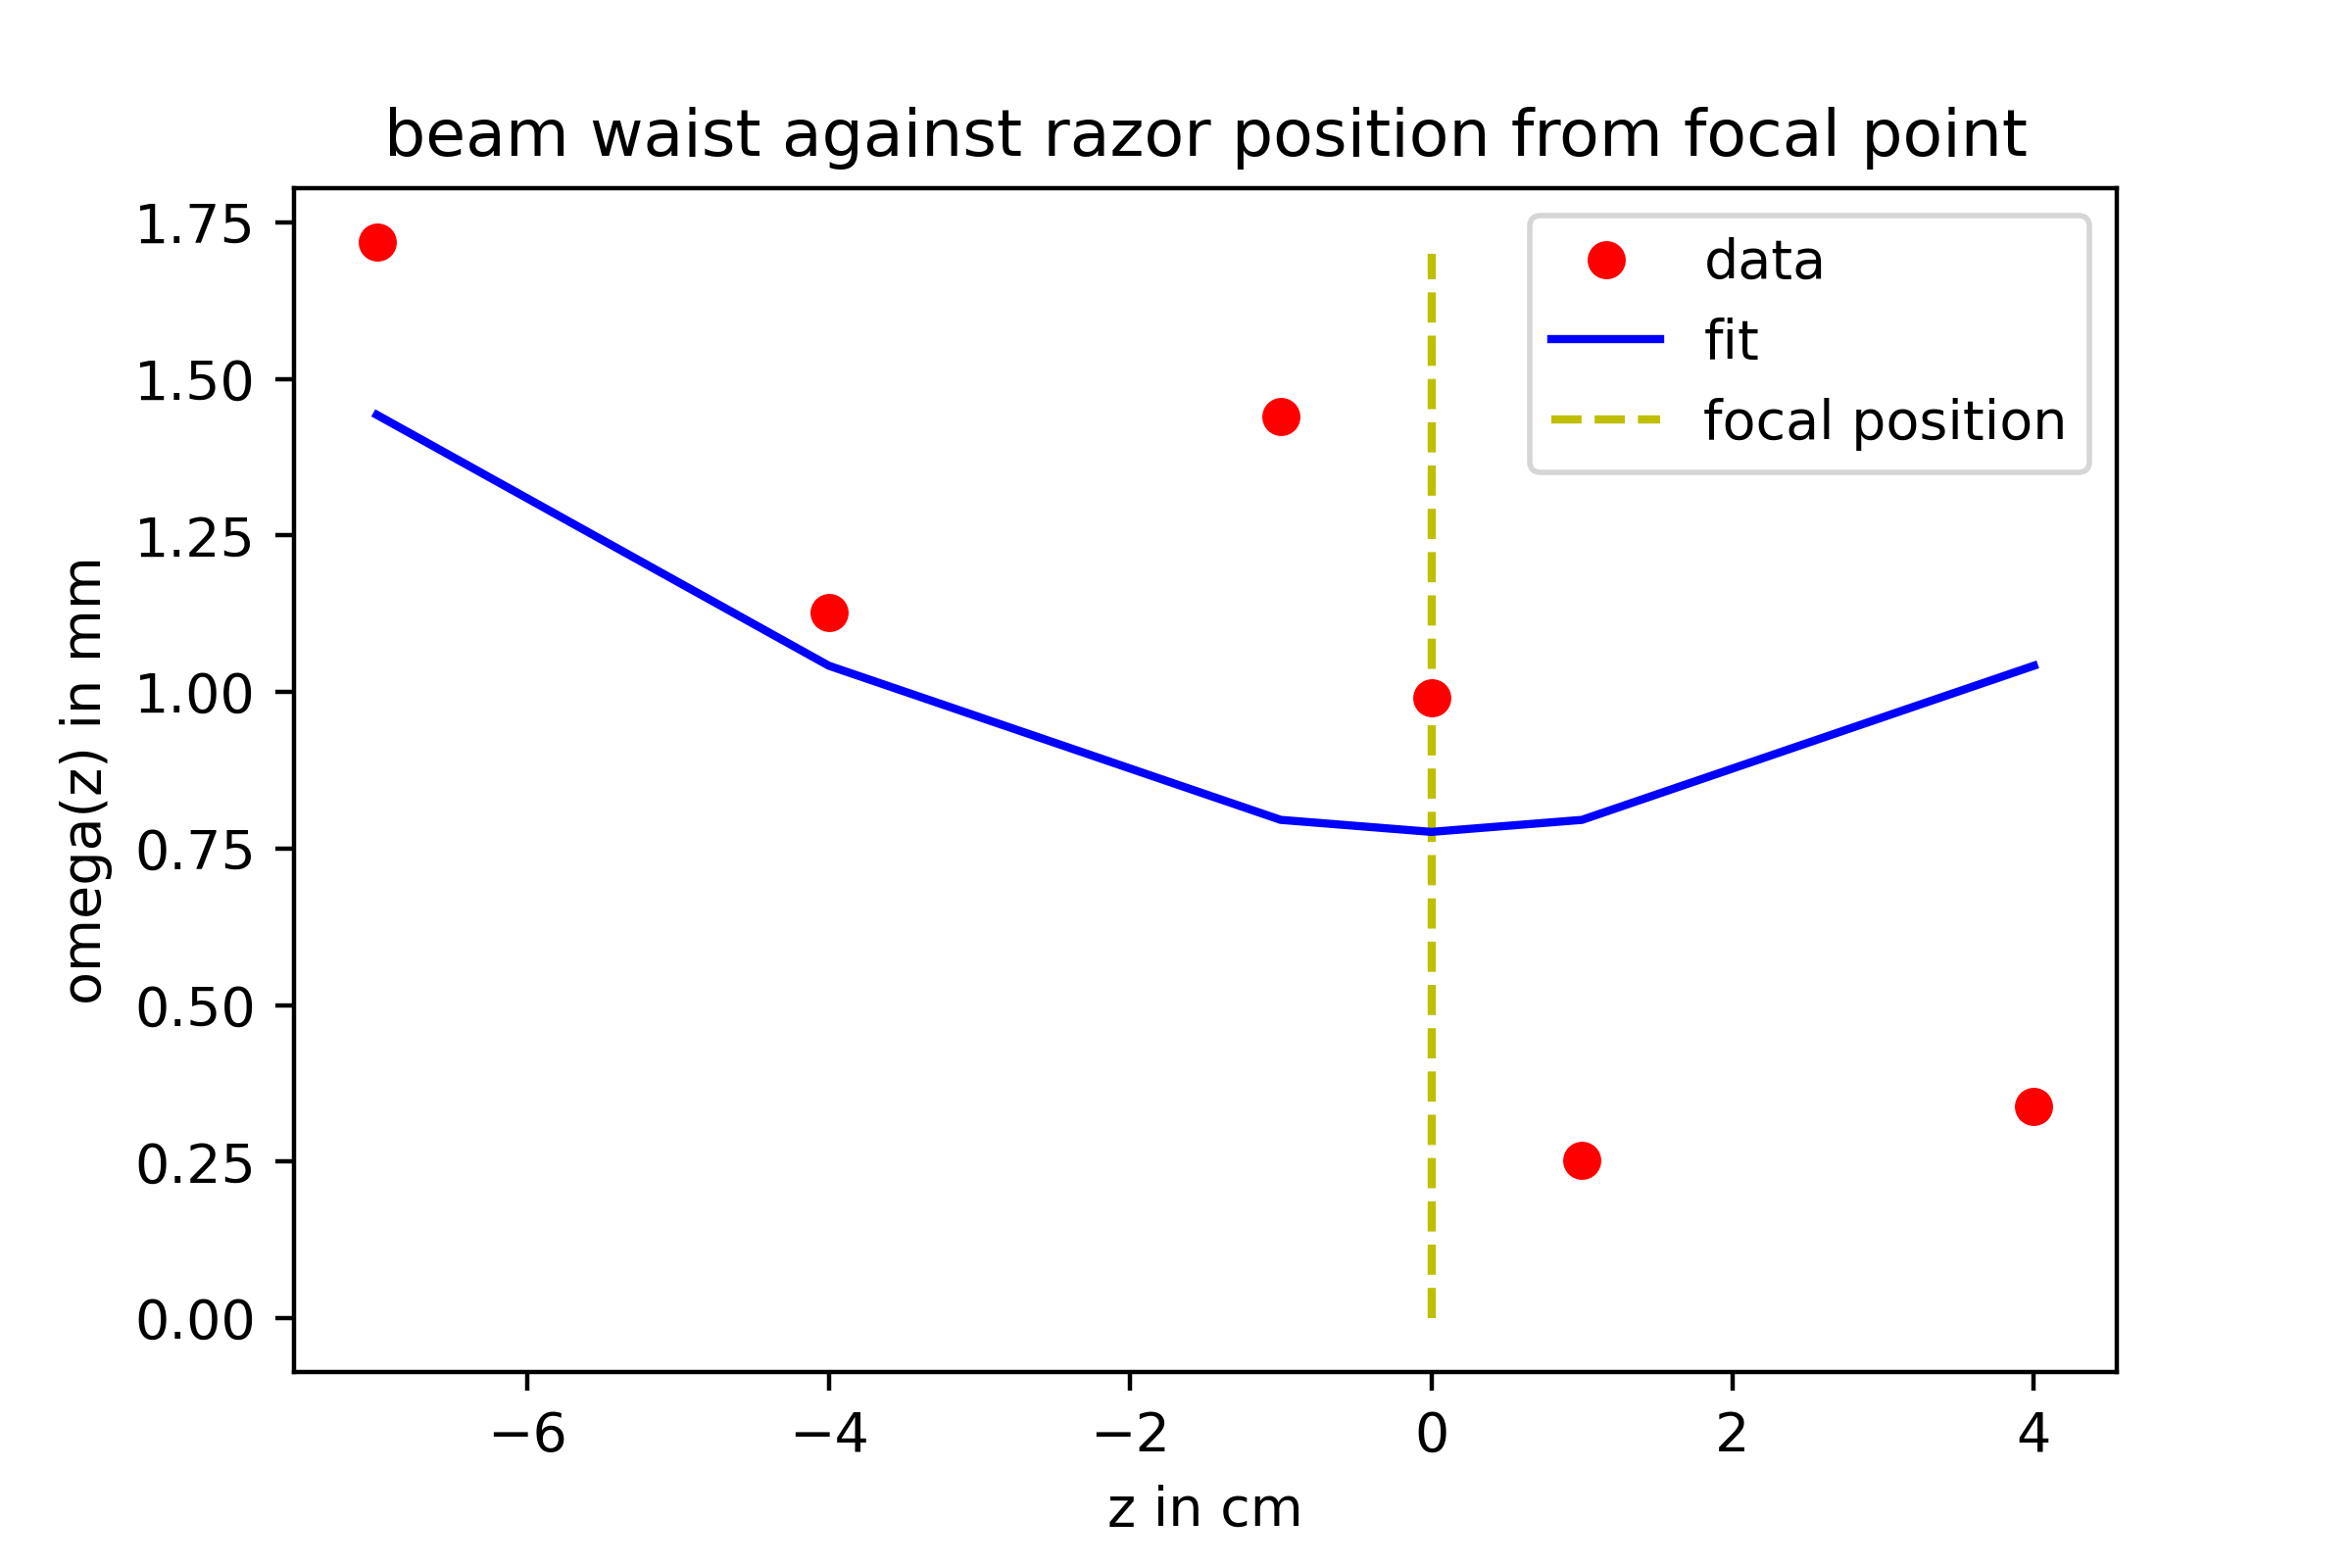
\includegraphics[width=\textwidth]{beam waist against razor position from focal point.png}[h!]

As in the previous part, we see that the standard deviations of $\omega_{0}$ and $z_{R}$ are relatively high. This time for the rayleigh length is is even higher than the value itself, which is illogical because it includes negative values within the error range. Since the experiments are very similar, the discussed error sources apply as well here. Furthermore, we observed extreme fluctuations on the multimeter display especially when measuring near the focal point. A reason for this could be that the waist is so small such that even the tiniest micrometer screw turn makes a lot of difference. In fact, sometimes only shoring softly on the table changed the displayed voltage by about 20 mV. To avoid abberations we made sure the beam enters the plano-convex lens on its curved surface, such that the refraction takes place on both surfaces of the lens. Nevertheless we could only approximately determine the center of the lens and thereby abberations can not be excluded totally.

\section{Optical resonator}

\begin{figure}[h!]
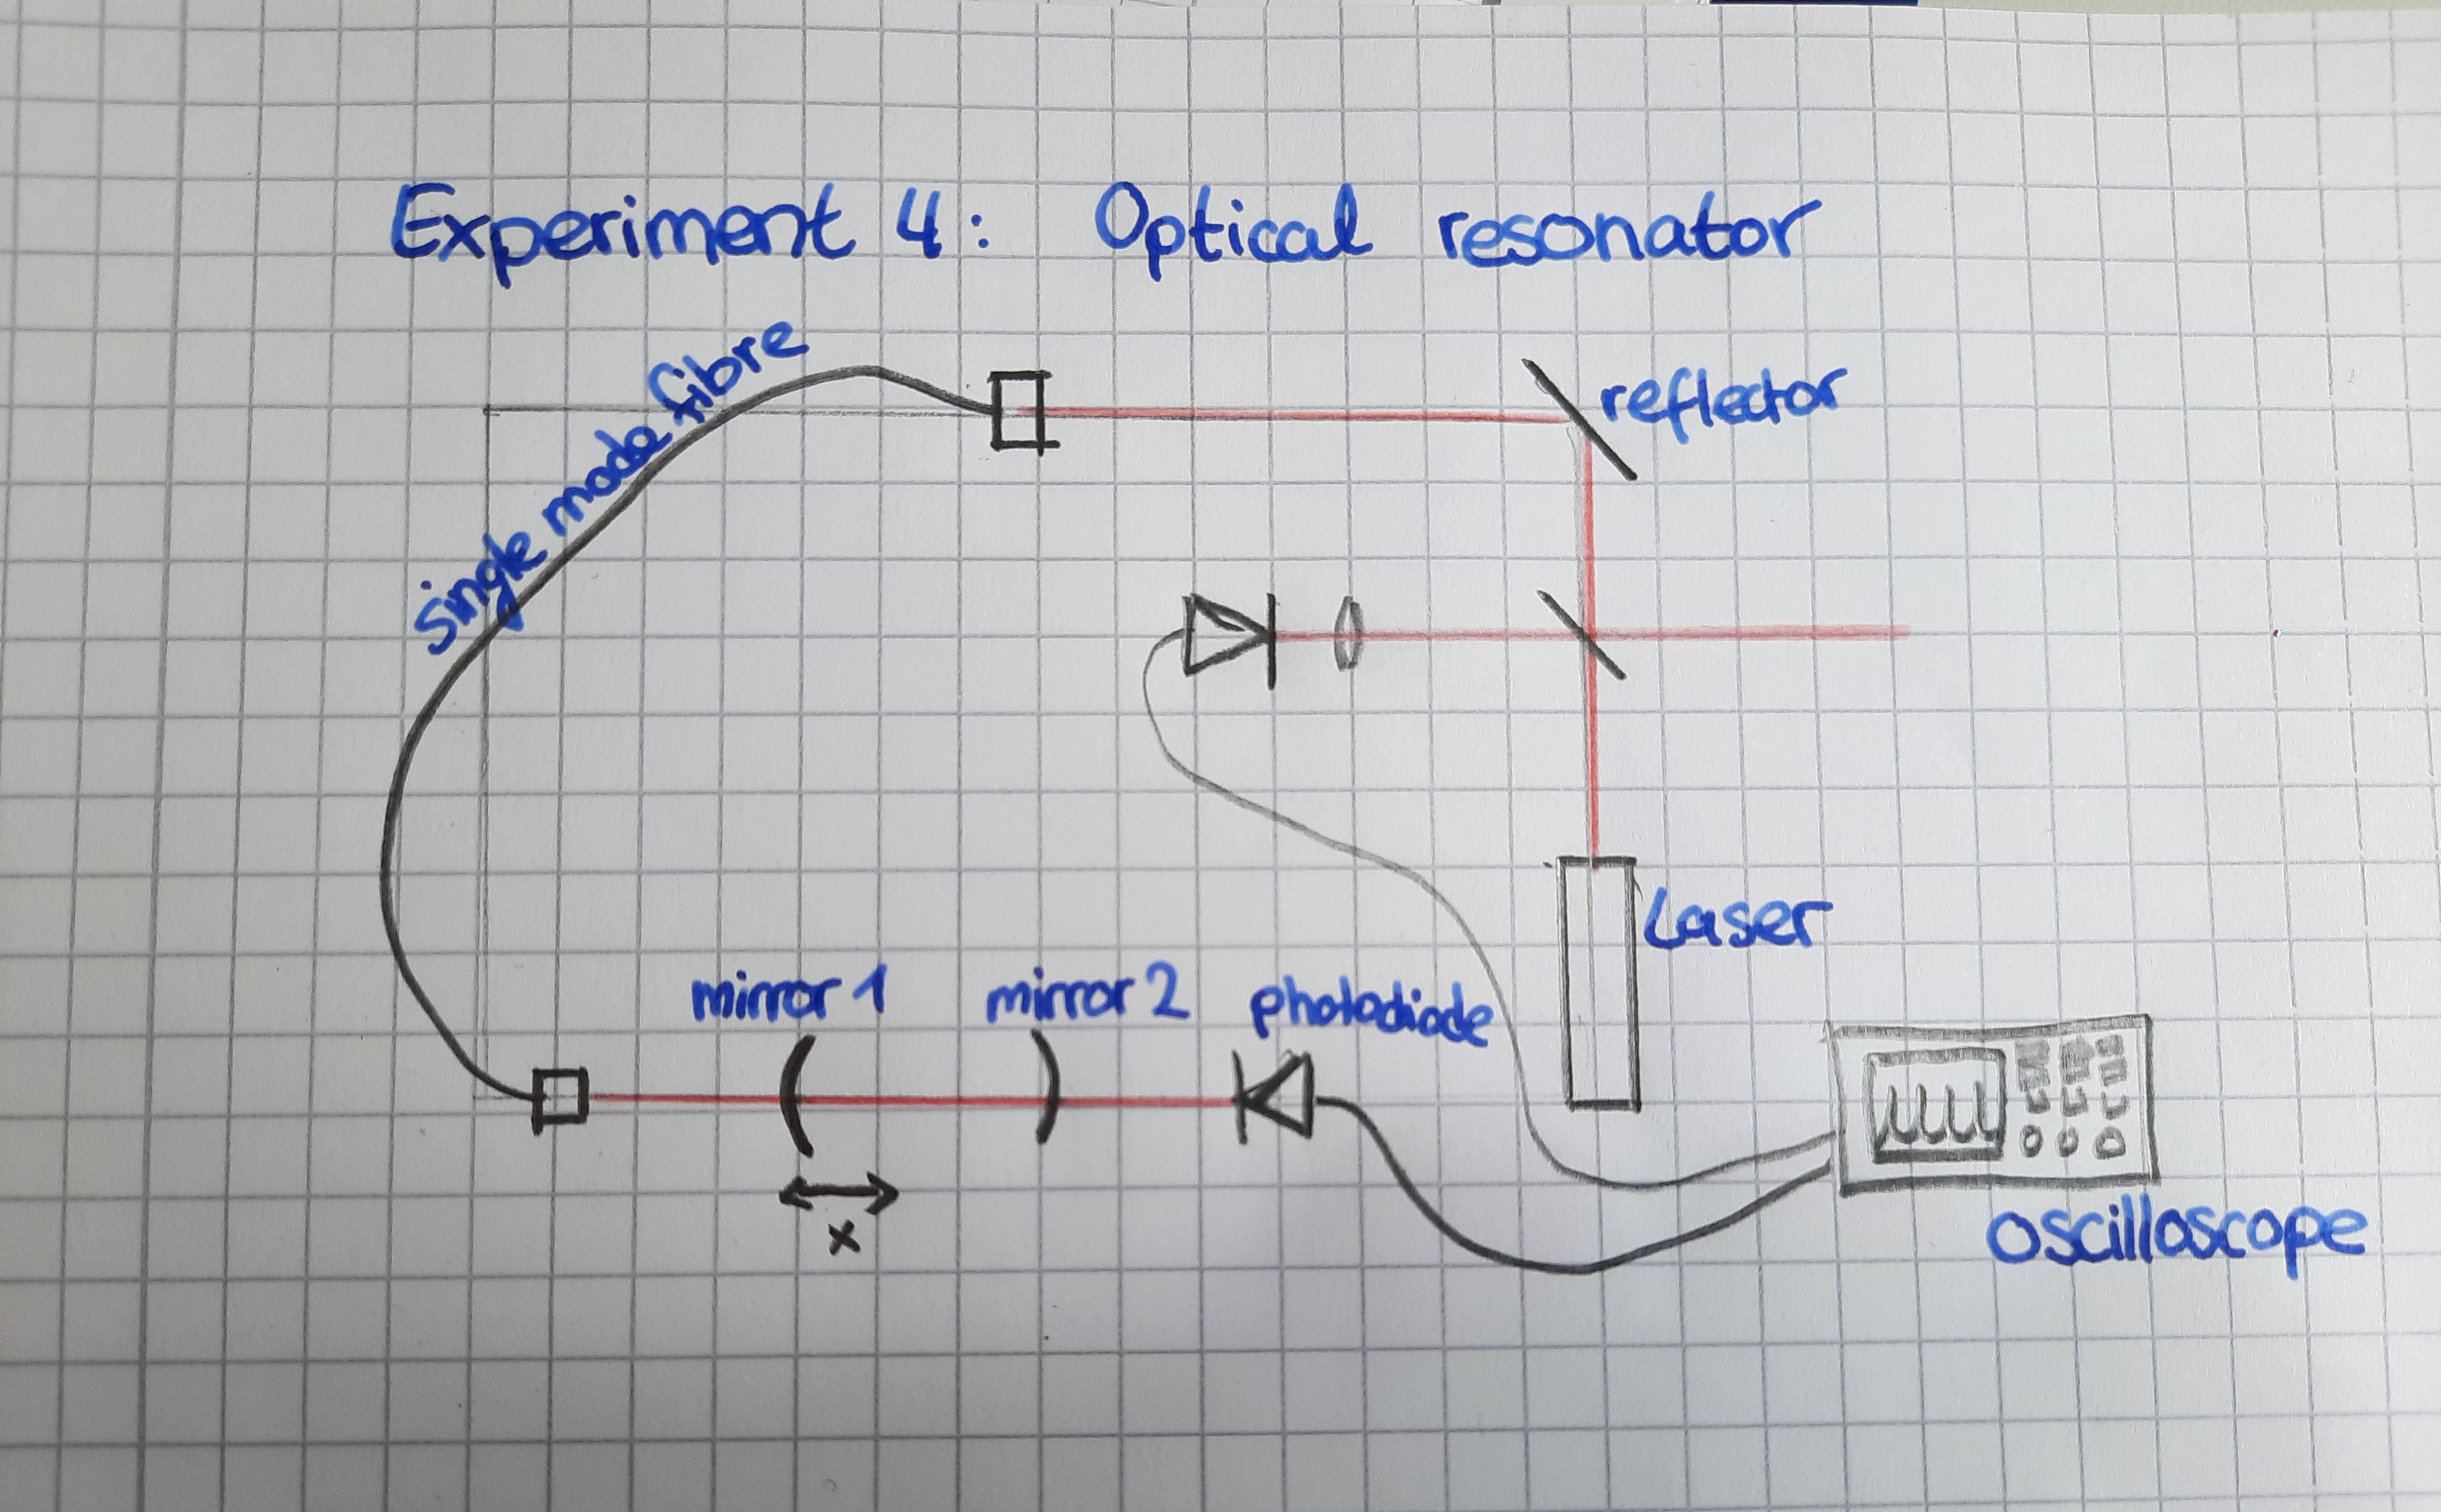
\includegraphics[width=\textwidth]{Tv4Aufbau.jpg}
\caption{Experiment 4: Optical resonator}
\label{TV4Aufbau}
\end{figure}

In the last part we constructed an optical resonator and detected the periodic signal of the beam that went through it with an oscilloscope. To do this we focused the beam on a lens 1 ($f=100mm$). Then we focused that on the movable reflector 1 with radius $r = 50mm$. In a distance $L=r$ (confocal arrangement) behind it we then positioned reflector 2 (same radius). The distance between lens 1 and reflector 1 is at first 50mm, so that the focal point of lens 1 lies exactly in the center of the optical resonator. At last we focused the beam into the center of a lens 2 and then into the photodiode with $R=100k\Omega$ (such that the signal is stronger), which we connected to the oscilloscope.

\paragraph{Determining the transmission of the two reflectors}
The mirrors of the Fabry-Perot-interferometer both let some of the incoming beam intensity pass and reflect some. A small amount might also be absorbed by the material of the mirror.\\

The transmittivity is then the intensity of the transmitted light divided by the intensity of the incoming light:
\begin{equation}
T = \frac{U_{t}}{U_{in}}
\label{transmittivitybyvoltage}
\end{equation}

The opposite of the transmissivity $T$ is the reflectivity $R$, if we assume that no light is absorbed by the mirrors they fulfil $R+T=1$. The total transmittivity can be calculated from the transmittivities of the single mirrors by $T = \sqrt{T_{1}T_{2}}$, and analogously  $R = \sqrt{R_{1}R_{2}}$. Having the reflectivity, we can calculate the finesse $F$, a measurement for the quality of the resonator:

\begin{equation}
F= \frac{\pi\sqrt{R}}{1-R}
\end{equation}

We measured the following:\\
$U_b = (29\pm1)mV$ voltage with both mirrors\\
$U_1 = (55\pm1)mV$  Spiegel voltage with first mirror\\
$U_2 = (46\pm1)mV$  voltage with second mirror\\
$U_o = (472\pm1)mV$ voltage without mirrors\\

From that we obtain \\

\begin{table}[H]
\centering
\begin{tabular}{|p{2cm}|p{3cm}|p{6cm}|}
\hline
Measurement & ... & Value \\
\hline
\multirow{1}{*}{Transmissivity}
        &Total Transmission & $T= T= 0.06144067796610169 \pm 0.00021226391960195743$\\
        &Transmission of first mirror & $T_{1}= 0.11652542372881355 \pm 0.00021226391960195743$\\
        &Transmission of second mirror & $T_{2}= 0.09745762711864406 \pm 0.00021226391960195743$\\
        &Total Transmission from $T_{1}$ and $T_{2}$& $T' = 0.10656590118609569 \pm 0.00021226391960195743$\\
\hline
\multirow{1}{*}{Reflectivity ($R=1-T$)}
        & R  &$R=  0.9385593220338984 \pm 0.00021226391960195743$\\
        & R' &$R'=  0.8934340988139043 \pm 1.724414796502769e-06$\\
        & Reflectivity of the first mirror &$ R1=  0.8834745762711864 \pm 0.00021329792298309015$\\
        & Reflectivity of the second mirror  &$R2=  0.902542372881356 \pm 0.00021286817188630018$\\
\hline
\multirow{1}{*}{Finesse}
        & Finesse from total R & $F= 49.5364337247994$\\
        & Finesse from R' & $F' = 27.865245432916524$ \\
\hline
\end{tabular}
\end{table}
%https://de.wikibooks.org/wiki/LaTeX-Kompendium:_Tabellen

From the signal detected by the oszilloscope (figure \ref{Osz1}) we can also determine the Finesse $F$. The full width at half maximum $\Delta\omega_{FWHM}$ and the free spectral range $\Delta\omega_{FSR}$, which is the distance of two peaks, are related by 
\begin{equation}
\Delta\omega_{FWHM} = \frac{\Delta\omega_{FSR}}{F}
\label{FinesseOszilloskopbild}
\end{equation}
Using the cursors, we see that the full width at half maximum is $\Delta\omega_{FWHM} =3 \pm 1$ units of the oszilloscope pattern. For the free spectral range we see that it is $\Delta\omega_{FSR} = 10 \pm 1$ units wide. Therefore we get a Finesse:\\
$F_{fig} = 3.3 \pm 1.1$\\
This is a very low value compared to the calculated values. As typical finesses are from 10 to up to 100000 \cite{optres} we expect the calculated values to be more accurate. Zooming into the peak of the oscilloscope would probably improve the resolution of the peak and thus lead to a better reading of the signal.\\

\begin{figure}[H]
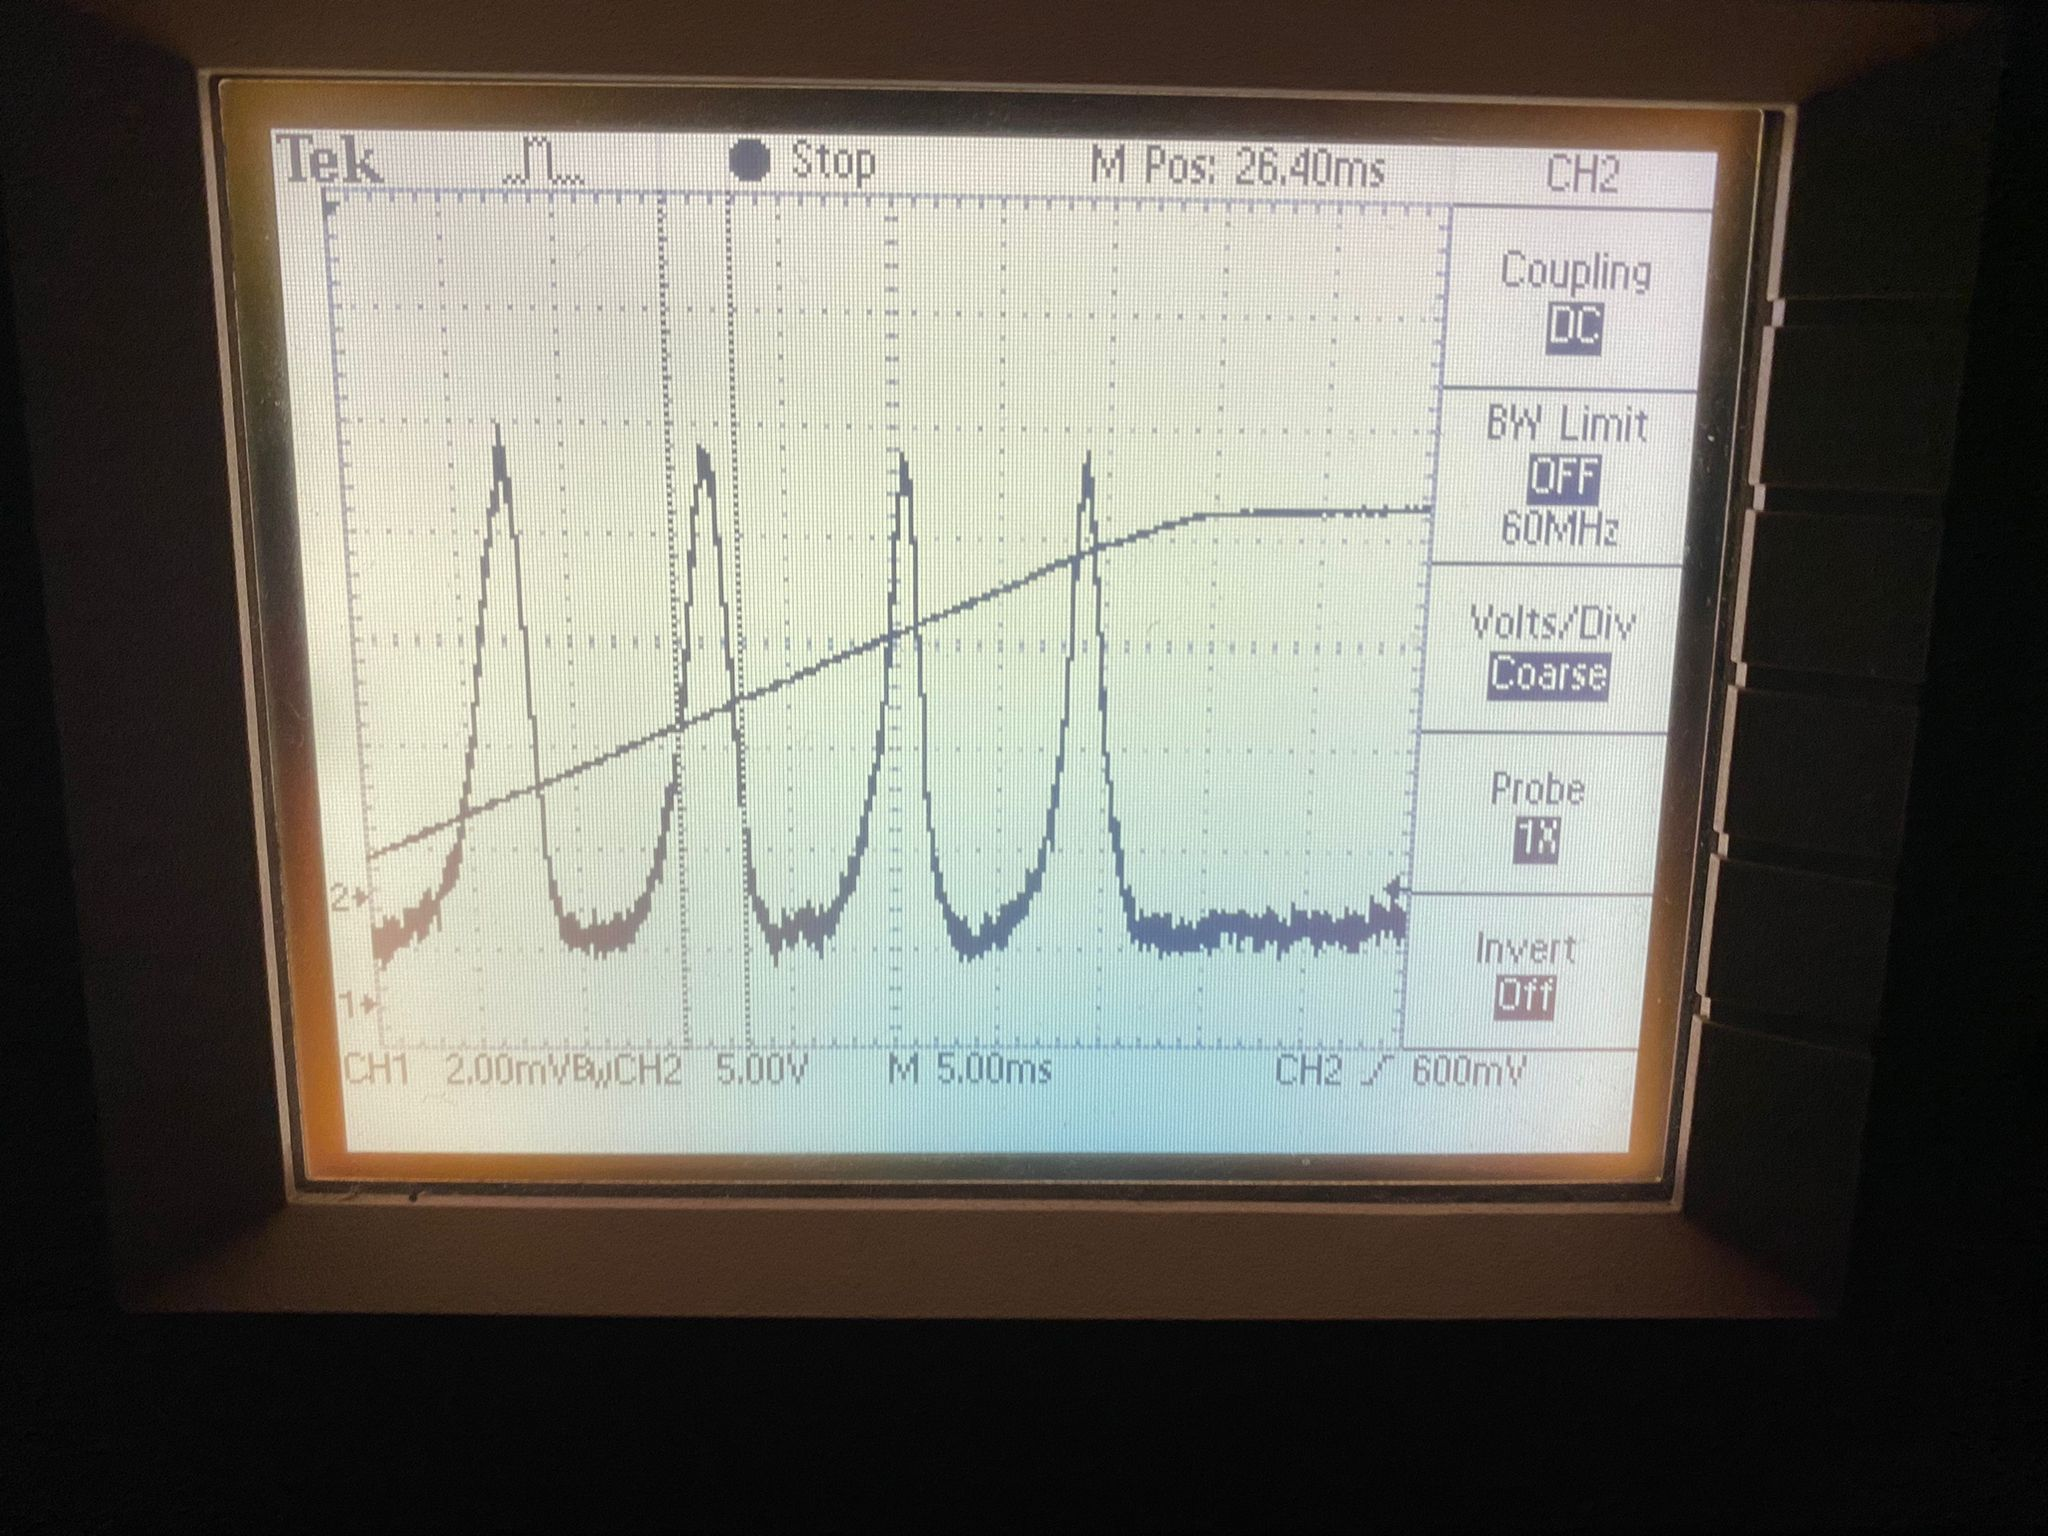
\includegraphics[width=\textwidth]{oszilloskopbild.jpg}
\caption{Oscilloscope image}
\label{Osz1}
\end{figure}

\begin{comment}
The next figure \ref{Osz3} shows the oscilloscope signal of one single peak:
\begin{figure}[h!]
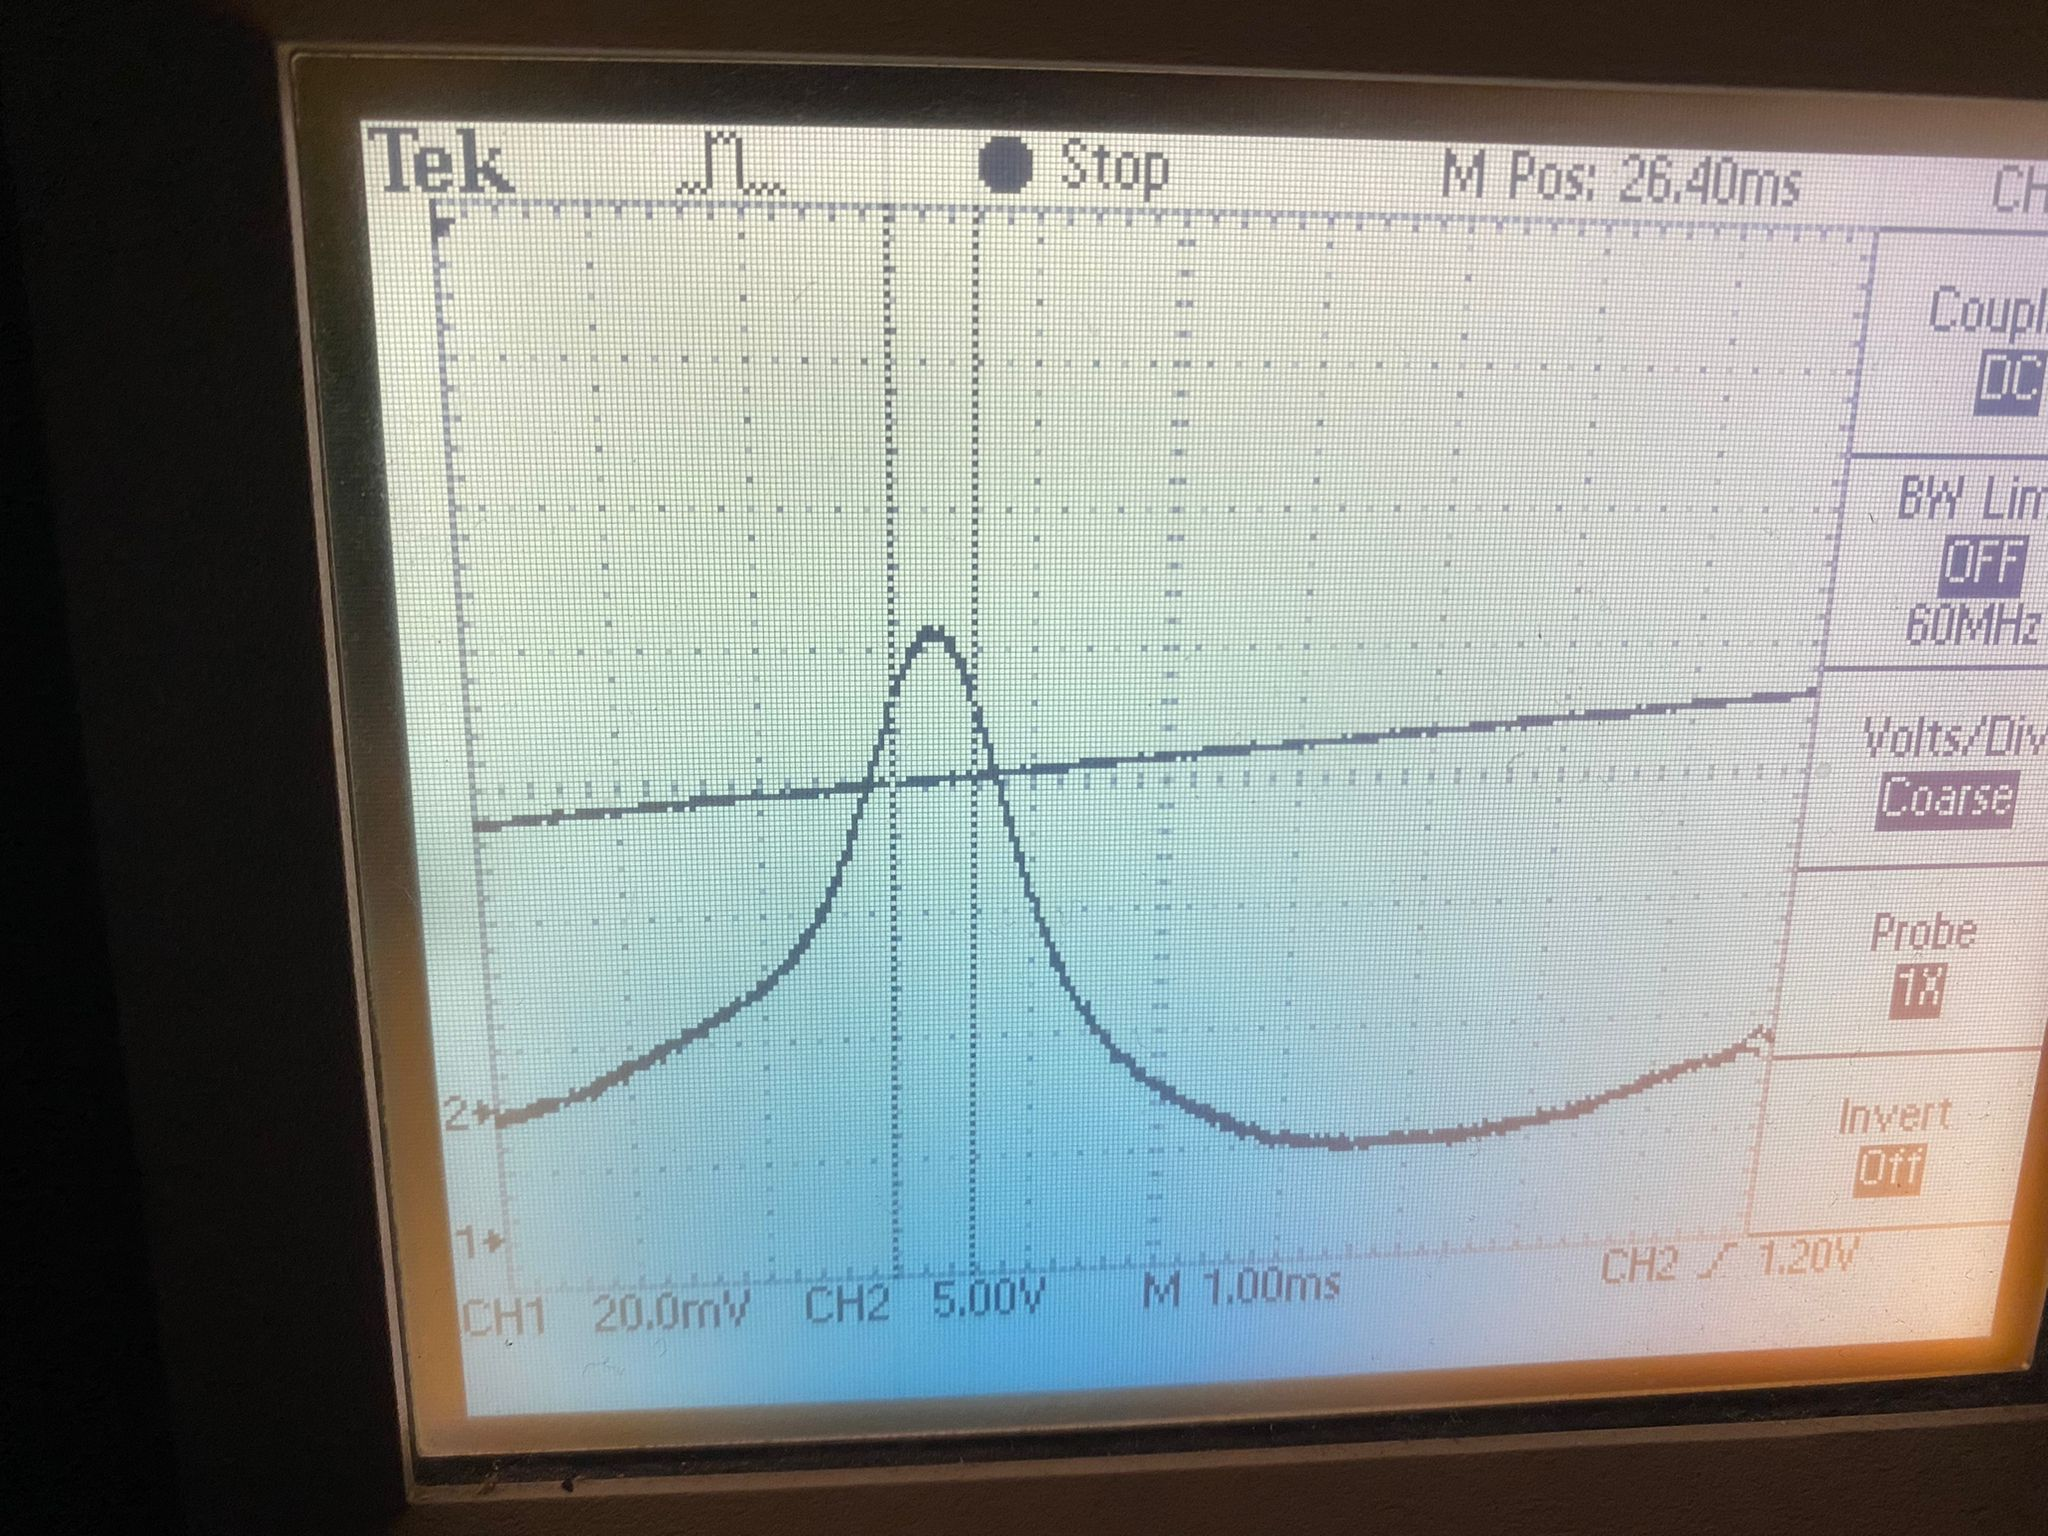
\includegraphics[width=\textwidth]{oszilloskopbild 3.jpg}
\caption{Osz3}
\label{Osz3}
\end{figure}
\end{comment}

In the following figure \ref{Eigenmoden_laser} we observe that between the peaks of the modes there are smaller modes which presumably depict the eigenmodes of the laser:
\textcolor{red}{Macht das Sinn?} \\

\begin{figure}[H]
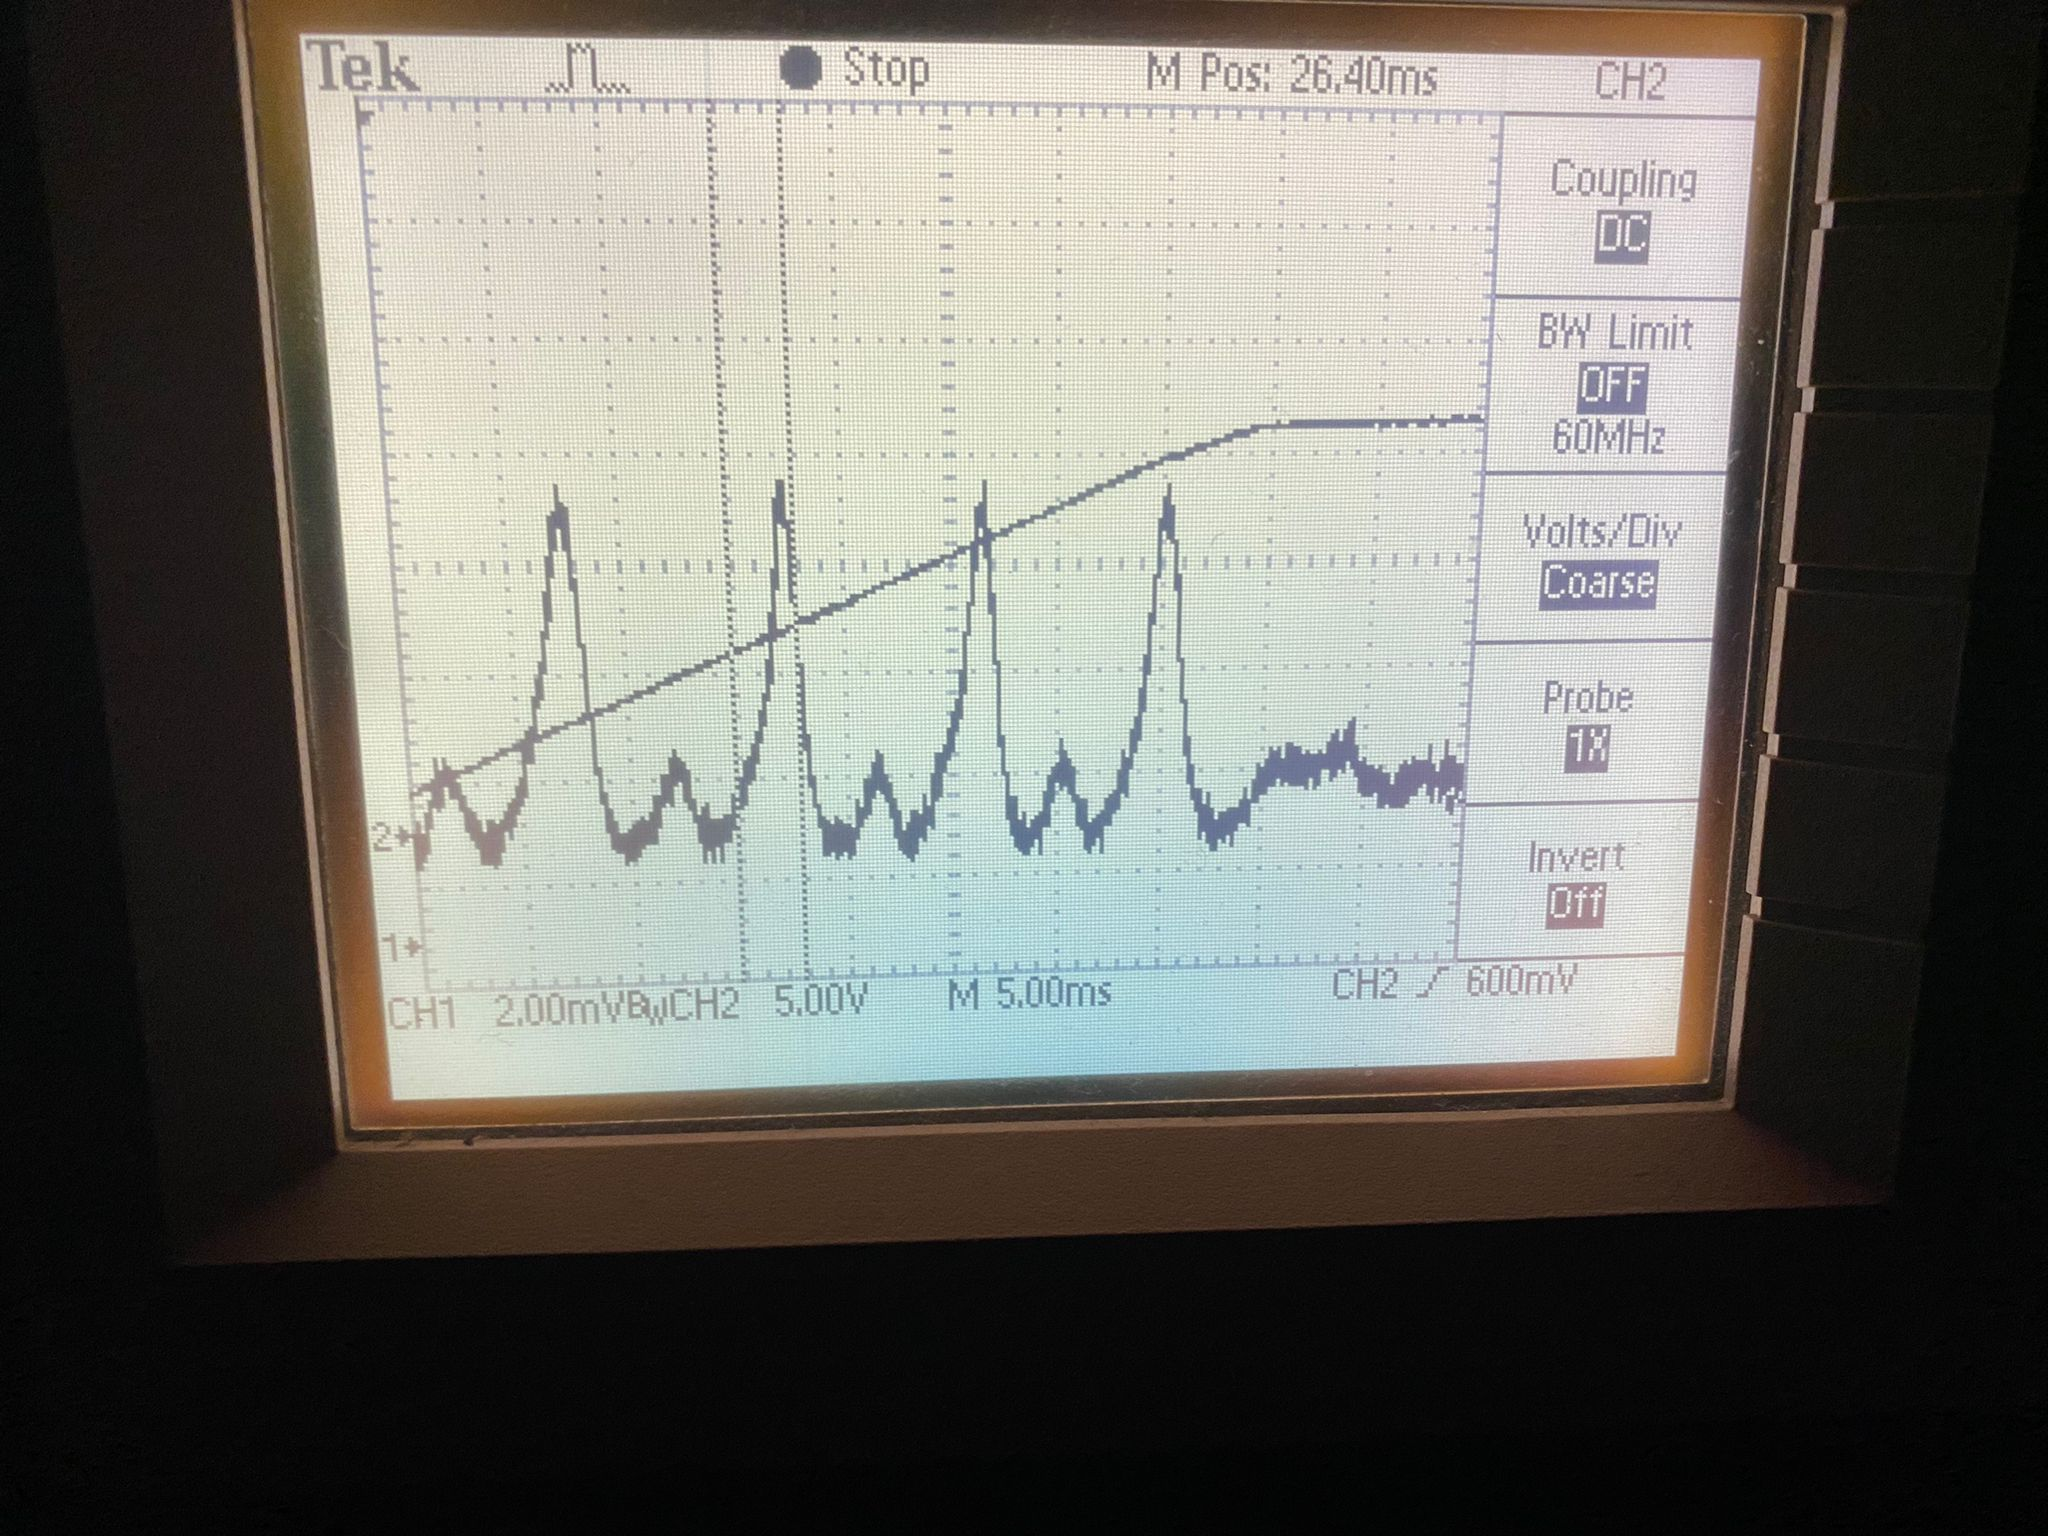
\includegraphics[width=\textwidth]{oszilloskopbild_mit_eigenmoden_vom_laser.jpg}
\caption{Other oscilloscope image}
\label{Eigenmoden_laser}
\end{figure}

\begin{figure}[h!]
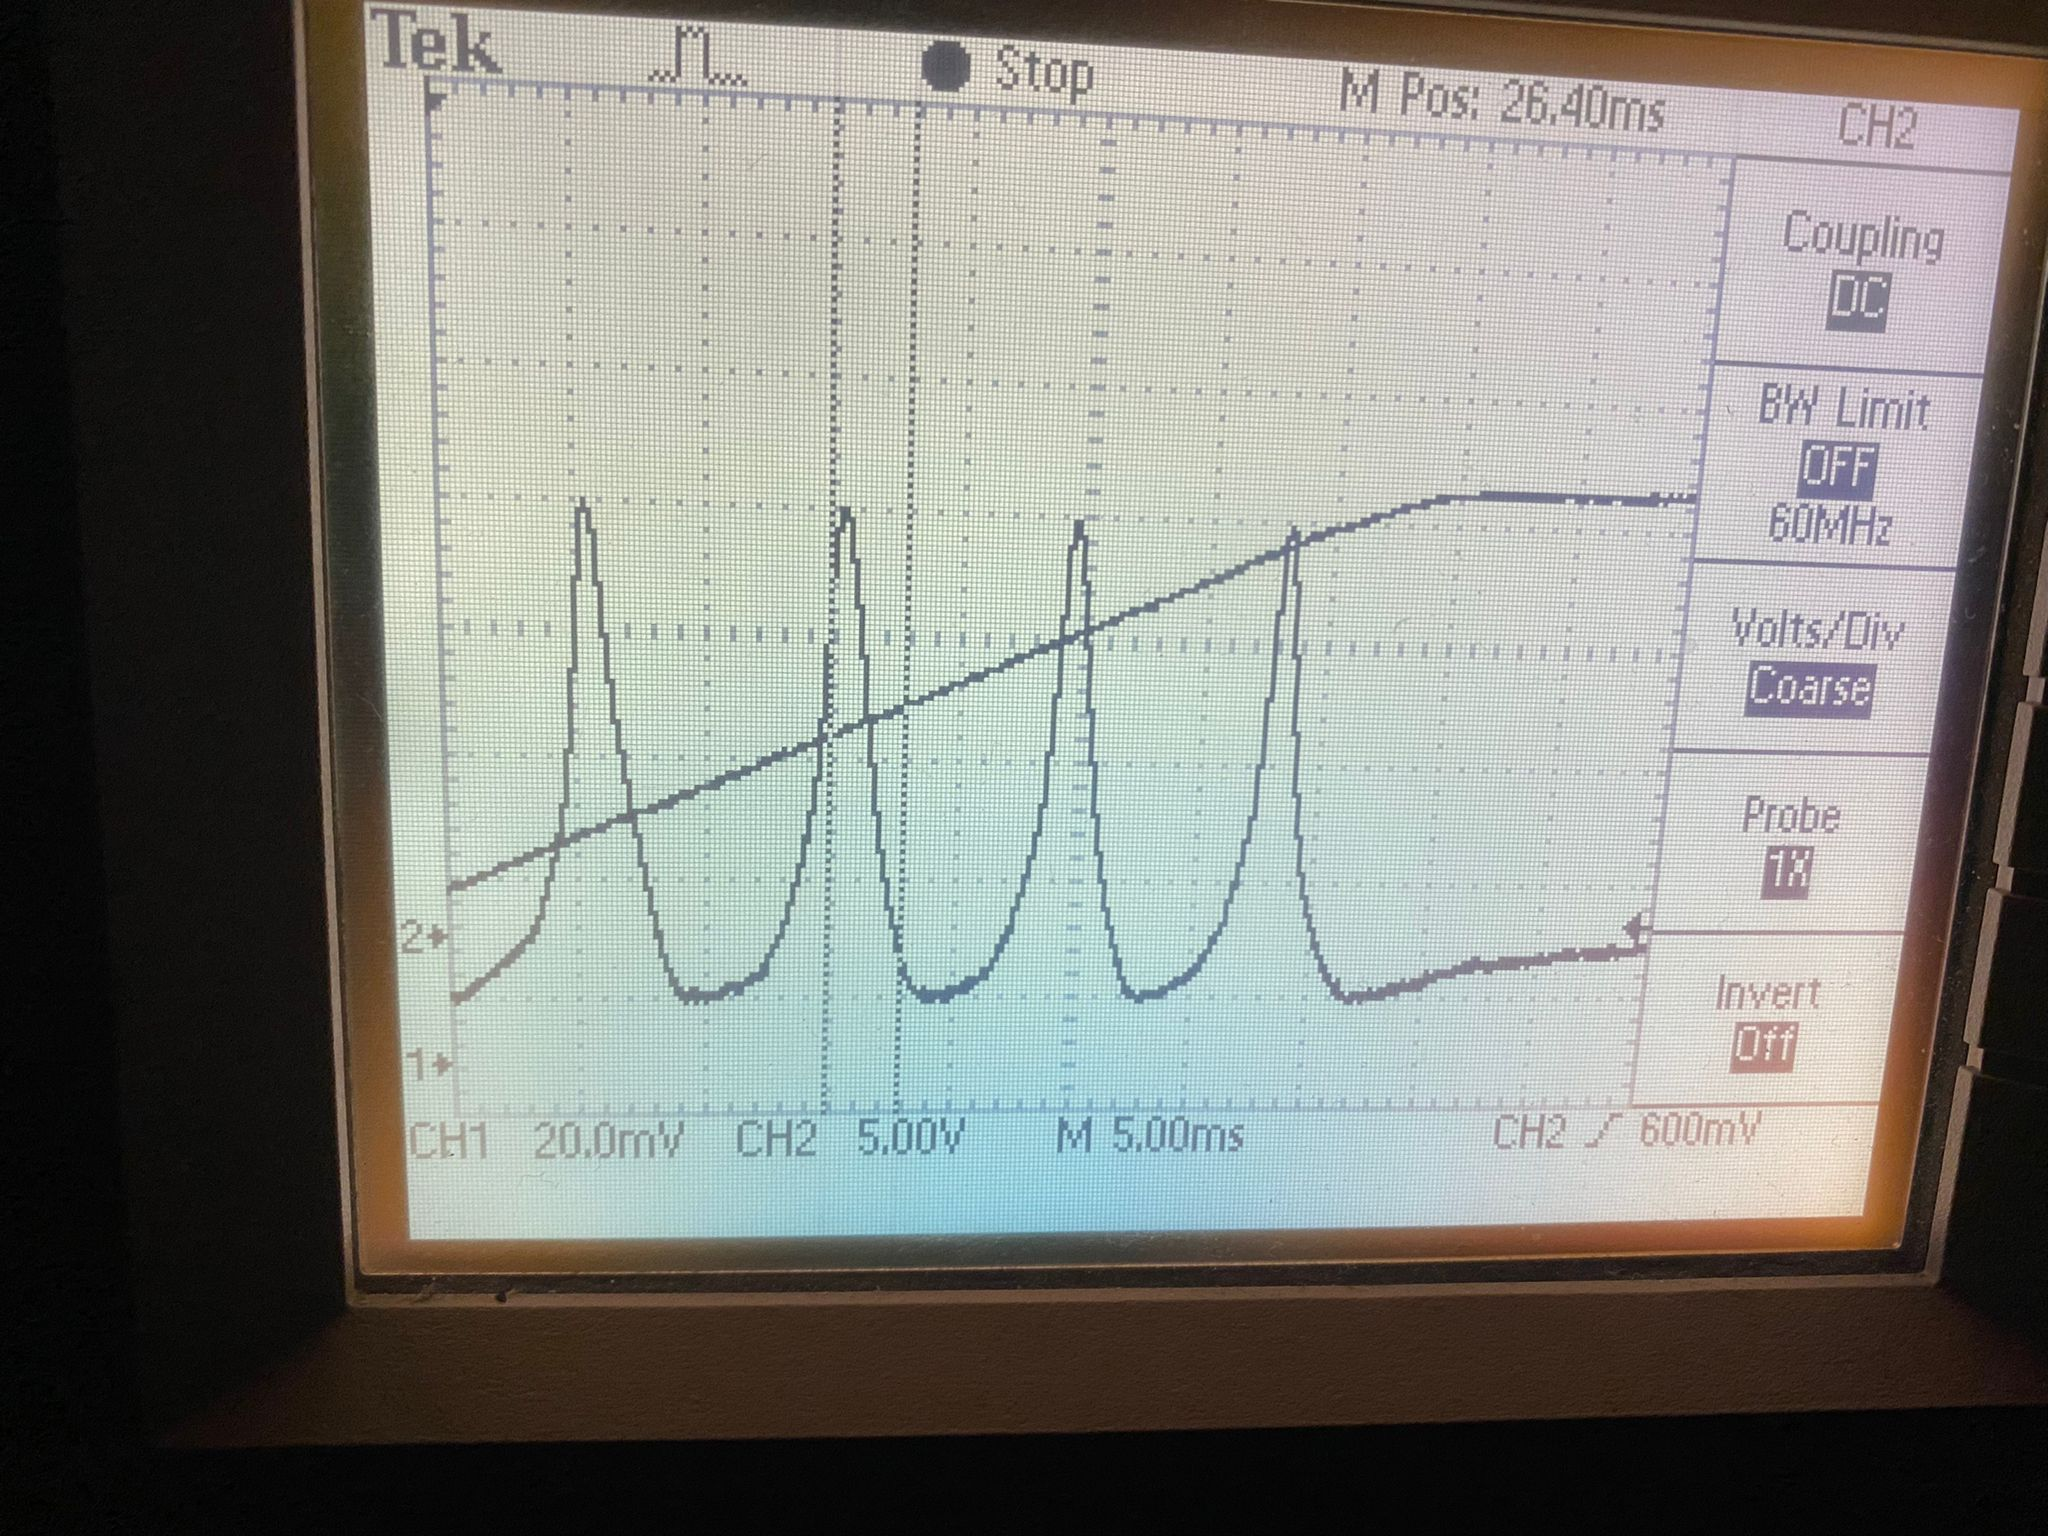
\includegraphics[width=\textwidth]{oszilloskopbild 2.jpg}
\caption{Another oscilloscope signal that we took}
\label{Osz2}
\end{figure}

We were also asked to check if the relation $T = \sqrt{T_{1}T_{2}}$ is valid. In the table above one can read the output values from the calculation program (see appendix). Comparing the Transmission: $T \approx (6.14 \pm 0.02) \cdot 10^{-2}$ with the Transmission from $T_{1}$ and $T_{2}$: $T' \approx (10.66 \pm 0.02) \cdot 10^{-2}$ we see that the difference is quite high and the margins of error do not overlap. Still, we assume that the relation can be confirmed. First, the errors were calculated from only the readoff-errors of the voltage (with Gauß' propagation of uncertainty law). However, there are more potential error sources as we have discussed in the previous lab report. Also, the values are close to another, compared to other measurements taken in the experiment. Some of the difference between the values can also be coming from the absorption of the reflector material, but we assume it is negligibly small.

\section{Appendix}

\subsection{Measurements}

\verbatiminput{Strahlprofil_a.csv}
\verbatiminput{Strahlprofil_b.csv}

\subsection{Pythoncode}

\lstset{literate=
  {á}{{\'a}}1 {é}{{\'e}}1 {í}{{\'i}}1 {ó}{{\'o}}1 {ú}{{\'u}}1
  {Á}{{\'A}}1 {É}{{\'E}}1 {Í}{{\'I}}1 {Ó}{{\'O}}1 {Ú}{{\'U}}1
  {à}{{\`a}}1 {è}{{\`e}}1 {ì}{{\`i}}1 {ò}{{\`o}}1 {ù}{{\`u}}1
  {À}{{\`A}}1 {È}{{\'E}}1 {Ì}{{\`I}}1 {Ò}{{\`O}}1 {Ù}{{\`U}}1
  {ä}{{\"a}}1 {ë}{{\"e}}1 {ï}{{\"i}}1 {ö}{{\"o}}1 {ü}{{\"u}}1
  {Ä}{{\"A}}1 {Ë}{{\"E}}1 {Ï}{{\"I}}1 {Ö}{{\"O}}1 {Ü}{{\"U}}1
  {â}{{\^a}}1 {ê}{{\^e}}1 {î}{{\^i}}1 {ô}{{\^o}}1 {û}{{\^u}}1
  {Â}{{\^A}}1 {Ê}{{\^E}}1 {Î}{{\^I}}1 {Ô}{{\^O}}1 {Û}{{\^U}}1
  {ã}{{\~a}}1 {ẽ}{{\~e}}1 {ĩ}{{\~i}}1 {õ}{{\~o}}1 {ũ}{{\~u}}1
  {Ã}{{\~A}}1 {Ẽ}{{\~E}}1 {Ĩ}{{\~I}}1 {Õ}{{\~O}}1 {Ũ}{{\~U}}1
  {œ}{{\oe}}1 {Œ}{{\OE}}1 {æ}{{\ae}}1 {Æ}{{\AE}}1 {ß}{{\ss}}1
  {ű}{{\H{u}}}1 {Ű}{{\H{U}}}1 {ő}{{\H{o}}}1 {Ő}{{\H{O}}}1
  {ç}{{\c c}}1 {Ç}{{\c C}}1 {ø}{{\o}}1 {å}{{\r a}}1 {Å}{{\r A}}1
  {€}{{\euro}}1 {£}{{\pounds}}1 {«}{{\guillemotleft}}1
  {»}{{\guillemotright}}1 {ñ}{{\~n}}1 {Ñ}{{\~N}}1 {¿}{{?`}}1 {¡}{{!`}}1 
}

\textcolor{blue}{Problem from page 16 of the experimental introduction}\\
\lstinputlisting[language=python]{aufgabe16.py}


\textcolor{blue}{Problem from page 7 of the experimental introduction}\\
\lstinputlisting[language=python]{matrizenoptik.py}


\textcolor{blue}{Measuring the beam profile (a)}\\
\lstinputlisting[language=python]{Strahlprofil_a.py}
\textcolor{blue}{Measuring the beam profile (b)}\\
\lstinputlisting[language=python]{Strahlprofil_b.py}

\textcolor{blue}{Optical resonator}\\
\lstinputlisting[language=python]{optical_resonator_if_PpropU.py}

\subsection{References}

\begin{thebibliography}{9}
\bibitem{Quantenausbeute} Wikipedia "Quantenausbeute", \url{https://de.wikipedia.org/wiki/Quantenausbeute} 
\bibitem{optres} Wikipedia "Optischer Resonator", \url{https://de.wikipedia.org/wiki/Optischer_Resonator}
\end{thebibliography}

\end{document}